% Options for packages loaded elsewhere
\PassOptionsToPackage{unicode}{hyperref}
\PassOptionsToPackage{hyphens}{url}
%
\documentclass[
]{book}
\usepackage{amsmath,amssymb}
\usepackage{lmodern}
\usepackage{iftex}
\ifPDFTeX
  \usepackage[T1]{fontenc}
  \usepackage[utf8]{inputenc}
  \usepackage{textcomp} % provide euro and other symbols
\else % if luatex or xetex
  \usepackage{unicode-math}
  \defaultfontfeatures{Scale=MatchLowercase}
  \defaultfontfeatures[\rmfamily]{Ligatures=TeX,Scale=1}
\fi
% Use upquote if available, for straight quotes in verbatim environments
\IfFileExists{upquote.sty}{\usepackage{upquote}}{}
\IfFileExists{microtype.sty}{% use microtype if available
  \usepackage[]{microtype}
  \UseMicrotypeSet[protrusion]{basicmath} % disable protrusion for tt fonts
}{}
\makeatletter
\@ifundefined{KOMAClassName}{% if non-KOMA class
  \IfFileExists{parskip.sty}{%
    \usepackage{parskip}
  }{% else
    \setlength{\parindent}{0pt}
    \setlength{\parskip}{6pt plus 2pt minus 1pt}}
}{% if KOMA class
  \KOMAoptions{parskip=half}}
\makeatother
\usepackage{xcolor}
\usepackage{longtable,booktabs,array}
\usepackage{calc} % for calculating minipage widths
% Correct order of tables after \paragraph or \subparagraph
\usepackage{etoolbox}
\makeatletter
\patchcmd\longtable{\par}{\if@noskipsec\mbox{}\fi\par}{}{}
\makeatother
% Allow footnotes in longtable head/foot
\IfFileExists{footnotehyper.sty}{\usepackage{footnotehyper}}{\usepackage{footnote}}
\makesavenoteenv{longtable}
\usepackage{graphicx}
\makeatletter
\def\maxwidth{\ifdim\Gin@nat@width>\linewidth\linewidth\else\Gin@nat@width\fi}
\def\maxheight{\ifdim\Gin@nat@height>\textheight\textheight\else\Gin@nat@height\fi}
\makeatother
% Scale images if necessary, so that they will not overflow the page
% margins by default, and it is still possible to overwrite the defaults
% using explicit options in \includegraphics[width, height, ...]{}
\setkeys{Gin}{width=\maxwidth,height=\maxheight,keepaspectratio}
% Set default figure placement to htbp
\makeatletter
\def\fps@figure{htbp}
\makeatother
\setlength{\emergencystretch}{3em} % prevent overfull lines
\providecommand{\tightlist}{%
  \setlength{\itemsep}{0pt}\setlength{\parskip}{0pt}}
\setcounter{secnumdepth}{5}
\usepackage{textcomp}
% \usepackage{palatino}
\usepackage{booktabs}
\usepackage{unixode}
\usepackage{tikz, tikz-cd}
\usepackage{pgfplots}
\pgfplotsset{compat=1.18}
\usetikzlibrary{positioning}
\usepackage[catalan]{babel}
\usepackage[left=3.5cm, right=3.5cm, top=3.5cm, bottom=3.5cm]{geometry}
\usepackage{csquotes}
\DeclareQuoteStyle{catalan}{``}{''}{``}{''}
\usepackage{amsmath,amsthm,amssymb,amsfonts}
\usepackage[all]{xy}
\usepackage{mathsymbols}

\addto\captionscatalan{\renewcommand{\chaptername}{Episodi}}

\definecolor{VerbatimBorderColor}{rgb}{0.7,0.7,0.7}
% from sphinxmanual.cls: put authors on separate lines
\DeclareRobustCommand{\and}{%
\end{tabular}\kern-\tabcolsep\\\begin{tabular}[t]{c}%
}

\usepackage{titlesec}
\titleformat{\chapter}[hang] 
{\normalfont\huge\bfseries}{\chaptertitlename\ \thechapter:}{.5em}{} 


%%%%%%%%%%%%%%%%%%%%%%%%%%%%

\usepackage{enumitem} % Customize lists
\setlist{nolistsep} % Reduce spacing between bullet points and numbered lists

\usepackage{booktabs} % Required for nicer horizontal rules in tables

\usepackage{xcolor} % Required for specifying colors by name
\definecolor{ocre}{RGB}{243,102,25} % Define the orange color used for highlighting throughout the book

%----------------------------------------------------------------------------------------
%	FONTS
%----------------------------------------------------------------------------------------

\usepackage[]{fontspec}
%\setromanfont{Latin Modern Math}
\setmathfont{Latin Modern Math}
\setsansfont{Bitstream Vera Sans}
\setmonofont{Bitstream Vera Sans Mono}

%\usepackage{palatino}
%\usepackage{avant} % Use the Avantgarde font for headings
%\usepackage{times} % Use the Times font for headings
% \usepackage{mathptmx} % Use the Adobe Times Roman as the default text font together with math symbols from the Sym­bol, Chancery and Com­puter Modern fonts
% \usepackage{libertine}
% \usepackage{noto}

\usepackage{microtype} % Slightly tweak font spacing for aesthetics
% \usepackage[utf8]{inputenc} % Required for including letters with accents
% \usepackage[T1]{fontenc} % Use 8-bit encoding that has 256 glyphs

%----------------------------------------------------------------------------------------
%	BIBLIOGRAPHY AND INDEX
%----------------------------------------------------------------------------------------

% \usepackage{csquotes}
\usepackage[style=alphabetic,citestyle=numeric,sorting=nyt,sortcites=true,autopunct=true,autolang=hyphen,hyperref=true,abbreviate=false,backref=true,backend=biber,defernumbers=true]{biblatex}
% \addbibresource{bibliografia.bib} % BibTeX bibliography file
% \defbibheading{bibempty}{}

% \usepackage{calc} % For simpler calculation - used for spacing the index letter headings correctly
% \usepackage{makeidx} % Required to make an index
% \makeindex % Tells LaTeX to create the files required for indexing

%----------------------------------------------------------------------------------------
%	MAIN TABLE OF CONTENTS
%----------------------------------------------------------------------------------------

\usepackage{titletoc} % Required for manipulating the table of contents

\contentsmargin{0cm} % Removes the default margin

% Part text styling
\titlecontents{part}[0cm]
{\addvspace{20pt}\centering\large\bfseries}
{}
{}
{}

% Chapter text styling
\titlecontents{chapter}[1.25cm] % Indentation
{\addvspace{12pt}\large\sffamily\bfseries} % Spacing and font options for chapters
{\color{ocre!60}\contentslabel[\Large\thecontentslabel]{1.25cm}\color{ocre}} % Chapter number
{\color{ocre}}  
{\color{ocre!60}\normalsize\;\titlerule*[.5pc]{.}\;\thecontentspage} % Page number

% Section text styling
\titlecontents{section}[1.25cm] % Indentation
{\addvspace{3pt}\sffamily\bfseries} % Spacing and font options for sections
{\contentslabel[\thecontentslabel]{1.25cm}} % Section number
{}
{\hfill\color{black}\thecontentspage} % Page number
[]

% Subsection text styling
\titlecontents{subsection}[1.25cm] % Indentation
{\addvspace{1pt}\sffamily\small} % Spacing and font options for subsections
{\contentslabel[\thecontentslabel]{1.25cm}} % Subsection number
{}
{\ \titlerule*[.5pc]{.}\;\thecontentspage} % Page number
[]

% List of figures
\titlecontents{figure}[0em]
{\addvspace{-5pt}\sffamily}
{\thecontentslabel\hspace*{1em}}
{}
{\ \titlerule*[.5pc]{.}\;\thecontentspage}
[]

% List of tables
\titlecontents{table}[0em]
{\addvspace{-5pt}\sffamily}
{\thecontentslabel\hspace*{1em}}
{}
{\ \titlerule*[.5pc]{.}\;\thecontentspage}
[]

%----------------------------------------------------------------------------------------
%	MINI TABLE OF CONTENTS IN PART HEADS
%----------------------------------------------------------------------------------------

% Chapter text styling
\titlecontents{lchapter}[0em] % Indenting
{\addvspace{15pt}\large\sffamily\bfseries} % Spacing and font options for chapters
{\color{ocre}\contentslabel[\Large\thecontentslabel]{1.25cm}\color{ocre}} % Chapter number
{}  
{\color{ocre}\normalsize\sffamily\bfseries\;\titlerule*[.5pc]{.}\;\thecontentspage} % Page number

% Section text styling
\titlecontents{lsection}[0em] % Indenting
{\sffamily\small} % Spacing and font options for sections
{\contentslabel[\thecontentslabel]{1.25cm}} % Section number
{}
{}

% Subsection text styling
\titlecontents{lsubsection}[.5em] % Indentation
{\normalfont\footnotesize\sffamily} % Font settings
{}
{}
{}

%----------------------------------------------------------------------------------------
%	PAGE HEADERS
%----------------------------------------------------------------------------------------

\usepackage{fancyhdr} % Required for header and footer configuration

\pagestyle{fancy}
\renewcommand{\chaptermark}[1]{\markboth{\sffamily\normalsize\bfseries\chaptername\ \thechapter.\ #1}{}} % Chapter text font settings
\renewcommand{\sectionmark}[1]{\markright{\sffamily\normalsize\thesection\hspace{5pt}#1}{}} % Section text font settings
\fancyhf{} \fancyhead[LE,RO]{\sffamily\normalsize\thepage} % Font setting for the page number in the header
\fancyhead[LO]{\rightmark} % Print the nearest section name on the left side of odd pages
\fancyhead[RE]{\leftmark} % Print the current chapter name on the right side of even pages
\renewcommand{\headrulewidth}{0.5pt} % Width of the rule under the header
\addtolength{\headheight}{2.5pt} % Increase the spacing around the header slightly
\renewcommand{\footrulewidth}{0pt} % Removes the rule in the footer
\fancypagestyle{plain}{\fancyhead{}\renewcommand{\headrulewidth}{0pt}} % Style for when a plain pagestyle is specified

% Removes the header from odd empty pages at the end of chapters
\makeatletter
\renewcommand{\cleardoublepage}{
\clearpage\ifodd\c@page\else
\hbox{}
\vspace*{\fill}
\thispagestyle{empty}
\newpage
\fi}

%----------------------------------------------------------------------------------------
%	THEOREM STYLES
%----------------------------------------------------------------------------------------

\usepackage{amsmath,amsfonts,amssymb,amsthm} % For math equations, theorems, symbols, etc

\newcommand{\intoo}[2]{\mathopen{]}#1\,;#2\mathclose{[}}
\newcommand{\ud}{\mathop{\mathrm{{}d}}\mathopen{}}
\newcommand{\intff}[2]{\mathopen{[}#1\,;#2\mathclose{]}}
\newtheorem{notation}{Notation}[chapter]

% Boxed/framed environments
\newtheoremstyle{ocrenumbox}% % Theorem style name
{0pt}% Space above
{0pt}% Space below
{\normalfont}% % Body font
{}% Indent amount
{\small\bf\sffamily\color{ocre}}% % Theorem head font
{\;}% Punctuation after theorem head
{0.25em}% Space after theorem head
{\small\sffamily\color{ocre}\thmname{#1}\nobreakspace\thmnumber{\@ifnotempty{#1}{}\@upn{#2}}% Theorem text (e.g. Theorem 2.1)
\thmnote{\nobreakspace\the\thm@notefont\sffamily\bfseries\color{black}---\nobreakspace#3.}} % Optional theorem note
\renewcommand{\qedsymbol}{$\blacksquare$}% Optional qed square

\newtheoremstyle{blacknumex}% Theorem style name
{5pt}% Space above
{5pt}% Space below
{\normalfont}% Body font
{} % Indent amount
{\small\bf\sffamily}% Theorem head font
{\;}% Punctuation after theorem head
{0.25em}% Space after theorem head
{\small\sffamily{\tiny\ensuremath{\blacksquare}}\nobreakspace\thmname{#1}\nobreakspace\thmnumber{\@ifnotempty{#1}{}\@upn{#2}}% Theorem text (e.g. Theorem 2.1)
\thmnote{\nobreakspace\the\thm@notefont\sffamily\bfseries---\nobreakspace#3.}}% Optional theorem note

\newtheoremstyle{blacknumbox} % Theorem style name
{0pt}% Space above
{0pt}% Space below
{\normalfont}% Body font
{}% Indent amount
{\small\bf\sffamily}% Theorem head font
{\;}% Punctuation after theorem head
{0.25em}% Space after theorem head
{\small\sffamily\thmname{#1}\nobreakspace\thmnumber{\@ifnotempty{#1}{}\@upn{#2}}% Theorem text (e.g. Theorem 2.1)
\thmnote{\nobreakspace\the\thm@notefont\sffamily\bfseries---\nobreakspace#3.}}% Optional theorem note

% Non-boxed/non-framed environments
\newtheoremstyle{ocrenum}% % Theorem style name
{5pt}% Space above
{5pt}% Space below
{\normalfont}% % Body font
{}% Indent amount
{\small\bf\sffamily\color{ocre}}% % Theorem head font
{\;}% Punctuation after theorem head
{0.25em}% Space after theorem head
{\small\sffamily\color{ocre}\thmname{#1}\nobreakspace\thmnumber{\@ifnotempty{#1}{}\@upn{#2}}% Theorem text (e.g. Theorem 2.1)
\thmnote{\nobreakspace\the\thm@notefont\sffamily\bfseries\color{black}---\nobreakspace#3.}} % Optional theorem note
\renewcommand{\qedsymbol}{$\blacksquare$}% Optional qed square
\makeatother



% Defines the theorem text style for each type of theorem to one of the three styles above
\newcounter{dummy} 
\numberwithin{dummy}{section}
\theoremstyle{ocrenumbox}
\newtheorem{theorem}[dummy]{TTTT}
\newtheorem{theoremeT}[dummy]{Teorema}
\newtheorem{problem}{Problema}[chapter]
\newtheorem{exerciseT}{Exercici}[chapter]
\theoremstyle{blacknumex}
\newtheorem{exampleT}{Exemple}[chapter]
\theoremstyle{blacknumbox}
\newtheorem{definitionT}{Definició}[section]
\newtheorem{corollaryT}[dummy]{Corol·lari}
\theoremstyle{ocrenum}
\newtheorem{propositionT}[dummy]{Proposició}
\newtheorem{lemmaT}[dummy]{Lema}

%----------------------------------------------------------------------------------------
%	DEFINITION OF COLORED BOXES
%----------------------------------------------------------------------------------------

\RequirePackage[framemethod=default]{mdframed} % Required for creating the theorem, definition, exercise and corollary boxes

% Theorem box
\newmdenv[skipabove=7pt,
skipbelow=7pt,
backgroundcolor=black!5,
linecolor=ocre,
innerleftmargin=5pt,
innerrightmargin=5pt,
innertopmargin=5pt,
leftmargin=0cm,
rightmargin=0cm,
innerbottommargin=5pt]{tBox}

% Proposition box
\newmdenv[skipabove=7pt,
skipbelow=7pt,
backgroundcolor=black!2,
linecolor=ocre,
innerleftmargin=5pt,
innerrightmargin=5pt,
innertopmargin=5pt,
leftmargin=0cm,
rightmargin=0cm,
innerbottommargin=5pt]{pBox}


% Exercise box	  
\newmdenv[skipabove=7pt,
skipbelow=7pt,
rightline=false,
leftline=true,
topline=false,
bottomline=false,
backgroundcolor=ocre!10,
linecolor=ocre,
innerleftmargin=5pt,
innerrightmargin=5pt,
innertopmargin=5pt,
innerbottommargin=5pt,
leftmargin=0cm,
rightmargin=0cm,
linewidth=4pt]{eBox}	

% Definition box
\newmdenv[skipabove=7pt,
skipbelow=7pt,
rightline=false,
leftline=true,
topline=false,
bottomline=false,
linecolor=ocre,
innerleftmargin=5pt,
innerrightmargin=5pt,
innertopmargin=0pt,
leftmargin=0cm,
rightmargin=0cm,
linewidth=4pt,
innerbottommargin=0pt]{dBox}	

% Corollary box
\newmdenv[skipabove=7pt,
skipbelow=7pt,
rightline=false,
leftline=true,
topline=false,
bottomline=false,
linecolor=gray,
backgroundcolor=black!5,
innerleftmargin=5pt,
innerrightmargin=5pt,
innertopmargin=5pt,
leftmargin=0cm,
rightmargin=0cm,
linewidth=4pt,
innerbottommargin=5pt]{cBox}

% Creates an environment for each type of theorem and assigns it a theorem text style from the "Theorem Styles" section above and a colored box from above
\renewenvironment{theorem}{\begin{tBox}\begin{theoremeT}}{\end{theoremeT}\end{tBox}}
\newenvironment{proposition}{\begin{pBox}\begin{propositionT}}{\end{propositionT}\end{pBox}}
\newenvironment{lemma}{\begin{pBox}\begin{lemmaT}}{\end{lemmaT}\end{pBox}}
\newenvironment{exercise}{\begin{eBox}\begin{exerciseT}}{\hfill{\color{ocre}\tiny\ensuremath{\blacksquare}}\end{exerciseT}\end{eBox}}				  
\newenvironment{definition}{\begin{dBox}\begin{definitionT}}{\end{definitionT}\end{dBox}}	
\newenvironment{example}{\begin{exampleT}}{\hfill{\tiny\ensuremath{\blacksquare}}\end{exampleT}}		
\newenvironment{corollary}{\begin{cBox}\begin{corollaryT}}{\end{corollaryT}\end{cBox}}	

%----------------------------------------------------------------------------------------
%	REMARK ENVIRONMENT
%----------------------------------------------------------------------------------------

\newenvironment{remark}{\par\vspace{10pt}\small % Vertical white space above the remark and smaller font size
\begin{list}{}{
\leftmargin=35pt % Indentation on the left
\rightmargin=25pt}\item\ignorespaces % Indentation on the right
\makebox[-2.5pt]{\begin{tikzpicture}[overlay]
\node[draw=ocre!60,line width=1pt,circle,fill=ocre!25,font=\sffamily\bfseries,inner sep=2pt,outer sep=0pt] at (-15pt,0pt){\textcolor{ocre}{R}};\end{tikzpicture}} % Orange R in a circle
\advance\baselineskip -1pt}{\end{list}\vskip5pt} % Tighter line spacing and white space after remark

%----------------------------------------------------------------------------------------
%	SECTION NUMBERING IN THE MARGIN
%----------------------------------------------------------------------------------------

\makeatletter
\renewcommand{\@seccntformat}[1]{\llap{\textcolor{ocre}{\csname the#1\endcsname}\hspace{1em}}}                    
\renewcommand{\section}{\@startsection{section}{1}{\z@}
{-4ex \@plus -1ex \@minus -.4ex}
{1ex \@plus.2ex }
{\normalfont\large\sffamily\bfseries}}
\renewcommand{\subsection}{\@startsection {subsection}{2}{\z@}
{-3ex \@plus -0.1ex \@minus -.4ex}
{0.5ex \@plus.2ex }
{\normalfont\sffamily\bfseries}}
\renewcommand{\subsubsection}{\@startsection {subsubsection}{3}{\z@}
{-2ex \@plus -0.1ex \@minus -.2ex}
{.2ex \@plus.2ex }
{\normalfont\small\sffamily\bfseries}}                        
\renewcommand\paragraph{\@startsection{paragraph}{4}{\z@}
{-2ex \@plus-.2ex \@minus .2ex}
{.1ex}
{\normalfont\small\sffamily\bfseries}}

%----------------------------------------------------------------------------------------
%	PART HEADINGS
%----------------------------------------------------------------------------------------

% numbered part in the table of contents
\newcommand{\@mypartnumtocformat}[2]{%
\setlength\fboxsep{0pt}%
\noindent\colorbox{ocre!20}{\strut\parbox[c][.7cm]{\ecart}{\color{ocre!70}\Large\sffamily\bfseries\centering#1}}\hskip\esp\colorbox{ocre!40}{\strut\parbox[c][.7cm]{\linewidth-\ecart-\esp}{\Large\sffamily\centering#2}}}%
%%%%%%%%%%%%%%%%%%%%%%%%%%%%%%%%%%
% unnumbered part in the table of contents
\newcommand{\@myparttocformat}[1]{%
\setlength\fboxsep{0pt}%
\noindent\colorbox{ocre!40}{\strut\parbox[c][.7cm]{\linewidth}{\Large\sffamily\centering#1}}}%
%%%%%%%%%%%%%%%%%%%%%%%%%%%%%%%%%%
\newlength\esp
\setlength\esp{4pt}
\newlength\ecart
\setlength\ecart{1.2cm-\esp}
\newcommand{\thepartimage}{}%
\newcommand{\partimage}[1]{\renewcommand{\thepartimage}{#1}}%
\def\@part[#1]#2{%
\ifnum \c@secnumdepth >-2\relax%
\refstepcounter{part}%
\addcontentsline{toc}{part}{\texorpdfstring{\protect\@mypartnumtocformat{\thepart}{#1}}{\partname~\thepart\ ---\ #1}}
\else%
\addcontentsline{toc}{part}{\texorpdfstring{\protect\@myparttocformat{#1}}{#1}}%
\fi%
\startcontents%
\markboth{}{}%
{\thispagestyle{empty}%
\begin{tikzpicture}[remember picture,overlay]%
\node at (current page.north west){\begin{tikzpicture}[remember picture,overlay]%	
\fill[ocre!20](0cm,0cm) rectangle (\paperwidth,-\paperheight);
\node[anchor=north] at (4cm,-3.25cm){\color{ocre!40}\fontsize{220}{100}\sffamily\bfseries\@Roman\c@part}; 
\node[anchor=south east] at (\paperwidth-1cm,-\paperheight+1cm){\parbox[t][][t]{8.5cm}{
\printcontents{l}{0}{\setcounter{tocdepth}{1}}%
}};
\node[anchor=north east] at (\paperwidth-1.5cm,-3.25cm){\parbox[t][][t]{15cm}{\strut\raggedleft\color{white}\fontsize{30}{30}\sffamily\bfseries#2}};
\end{tikzpicture}};
\end{tikzpicture}}%
\@endpart}
\def\@spart#1{%
\startcontents%
\phantomsection
{\thispagestyle{empty}%
\begin{tikzpicture}[remember picture,overlay]%
\node at (current page.north west){\begin{tikzpicture}[remember picture,overlay]%	
\fill[ocre!20](0cm,0cm) rectangle (\paperwidth,-\paperheight);
\node[anchor=north east] at (\paperwidth-1.5cm,-3.25cm){\parbox[t][][t]{15cm}{\strut\raggedleft\color{white}\fontsize{30}{30}\sffamily\bfseries#1}};
\end{tikzpicture}};
\end{tikzpicture}}
\addcontentsline{toc}{part}{\texorpdfstring{%
\setlength\fboxsep{0pt}%
\noindent\protect\colorbox{ocre!40}{\strut\protect\parbox[c][.7cm]{\linewidth}{\Large\sffamily\protect\centering #1\quad\mbox{}}}}{#1}}%
\@endpart}
\def\@endpart{\vfil\newpage
\if@twoside
\if@openright
\null
\thispagestyle{empty}%
\newpage
\fi
\fi
\if@tempswa
\twocolumn
\fi}

%----------------------------------------------------------------------------------------
%	CHAPTER HEADINGS
%----------------------------------------------------------------------------------------

% A switch to conditionally include a picture, implemented by  Christian Hupfer
\newif\ifusechapterimage
\usechapterimagetrue
\newcommand{\thechapterimage}{}%
\newcommand{\chapterimage}[1]{\ifusechapterimage\renewcommand{\thechapterimage}{#1}\fi}%
\def\@makechapterhead#1{%
{\parindent \z@ \raggedright \normalfont
\ifnum \c@secnumdepth >\m@ne
\if@mainmatter
\begin{tikzpicture}[remember picture,overlay]
\node at (current page.north west)
{\begin{tikzpicture}[remember picture,overlay]
\node[anchor=north west,inner sep=0pt] at (0,0) {\ifusechapterimage\includegraphics[width=\paperwidth]{\thechapterimage}\fi};
\draw[anchor=west] (\Gm@lmargin,-9cm) node [line width=2pt,rounded corners=15pt,draw=ocre,fill=white,fill opacity=0.5,inner sep=15pt]{\strut\makebox[22cm]{}};
\draw[anchor=west] (\Gm@lmargin+.3cm,-9cm) node {\huge\sffamily\bfseries\color{black}\thechapter. #1\strut};
\end{tikzpicture}};
\end{tikzpicture}
\else
\begin{tikzpicture}[remember picture,overlay]
\node at (current page.north west)
{\begin{tikzpicture}[remember picture,overlay]
\node[anchor=north west,inner sep=0pt] at (0,0) {\ifusechapterimage\includegraphics[width=\paperwidth]{\thechapterimage}\fi};
\draw[anchor=west] (\Gm@lmargin,-9cm) node [line width=2pt,rounded corners=15pt,draw=ocre,fill=white,fill opacity=0.5,inner sep=15pt]{\strut\makebox[22cm]{}};
\draw[anchor=west] (\Gm@lmargin+.3cm,-9cm) node {\huge\sffamily\bfseries\color{black}#1\strut};
\end{tikzpicture}};
\end{tikzpicture}
\fi\fi\par\vspace*{270\p@}}}

%-------------------------------------------

\def\@makeschapterhead#1{%
\begin{tikzpicture}[remember picture,overlay]
\node at (current page.north west)
{\begin{tikzpicture}[remember picture,overlay]
\node[anchor=north west,inner sep=0pt] at (0,0) {\ifusechapterimage\includegraphics[width=\paperwidth]{\thechapterimage}\fi};
\draw[anchor=west] (\Gm@lmargin,-9cm) node [line width=2pt,rounded corners=15pt,draw=ocre,fill=white,fill opacity=0.5,inner sep=15pt]{\strut\makebox[22cm]{}};
\draw[anchor=west] (\Gm@lmargin+.3cm,-9cm) node {\huge\sffamily\bfseries\color{black}#1\strut};
\end{tikzpicture}};
\end{tikzpicture}
\par\vspace*{270\p@}}
\makeatother

%----------------------------------------------------------------------------------------
%	HYPERLINKS IN THE DOCUMENTS
%----------------------------------------------------------------------------------------

\usepackage{hyperref}
\hypersetup{hidelinks,colorlinks=false,breaklinks=true,urlcolor= ocre,bookmarksopen=false,pdftitle={Title},pdfauthor={Author}}
\usepackage{bookmark}
\bookmarksetup{
open,
numbered,
addtohook={%
\ifnum\bookmarkget{level}=0 % chapter
\bookmarksetup{bold}%
\fi
\ifnum\bookmarkget{level}=-1 % part
\bookmarksetup{color=ocre,bold}%
\fi
}
}
\usepackage{textcomp}
\ifLuaTeX
  \usepackage{selnolig}  % disable illegal ligatures
\fi
\usepackage[]{biblatex}
\addbibresource{src/bibliografia.bib}
\nocite{geck, rotman, weintraub, zbigniew, dummitfoote, artinalgebra}
\IfFileExists{bookmark.sty}{\usepackage{bookmark}}{\usepackage{hyperref}}
\IfFileExists{xurl.sty}{\usepackage{xurl}}{} % add URL line breaks if available
\urlstyle{same} % disable monospaced font for URLs
\hypersetup{
  pdfauthor={Marc Masdeu},
  hidelinks,
  pdfcreator={LaTeX via pandoc}}

\author{Marc Masdeu}
\date{2023-02-15}

\begin{document}

%----------------------------------------------------------------------------------------
%	TITLE PAGE
%----------------------------------------------------------------------------------------

\begingroup
\thispagestyle{empty} % Suppress headers and footers on the title page
\begin{tikzpicture}[remember picture,overlay]
\node[inner sep=0pt] (background) at (current page.center) {};
\draw (current page.center) node [fill=ocre!30!white,fill opacity=0.6,text opacity=1,inner sep=1cm]{\Huge\centering\bfseries\sffamily\parbox[c][][t]{\paperwidth}{\centering Teoria de\\Galois\\[15pt] % Book title
{\Large Marc Masdeu, UAB}\\[10pt]
}};
\end{tikzpicture}


\vfill
\endgroup

\begin{center}
% https://tikzcd.yichuanshen.de/#N4Igdg9gJgpgziAXAbVABwnAlgFyxMJZAVgBoAGAXVJADcBDAGwFcYkQAdDgRW4AoucAI4AnHMgAsAX2AAmKaSwBKEAvSZc+QijIBGanSat2XXgI7CxchctWl12PASJlZBhizaJOPfrbUgGI5aLqQAzO5GXj68dg6azigAHKT6NB7G3qb8fLoAtMqCouISlNYqAUEJ2si65KmRnia+fLkA1IUWxZJl8nGBGk41AJykbulRzWZYRVbyFfYDwYnIsg0TTVktM11iPeX9VUNE9WmGmzH8syW9Ugvxxyi6Y42Zl+aWOAdSBjBQAObwIigABmIggAFskPUQDgIEhniAABYwehQdiQMBsAJgyHQmhwpApZGo9HeTHYxa4qGIGGExAAdhoKLRGIIlNB4JpiPpaxJrPJ7P61KQfPpYWZpLZWOFXKQo1h8MQEv5ZPAQpxcsZBKVCpZaopsrxiGJ9L1UsFMs1xrpSokkoF6qtVK1tqQZFV0o5IBFiHtiqQADYaIwsDLvHAIKH0Q6DUKCfQsIwvSAQ-QAEYwRgABUGIW8jBgIJwRppHvpwc9lu9vsr4tjKZ+UiAA
\begin{tikzcd}[column sep=small, row sep=large]
  &                                      &                                         &  &  & {\QQ(\sqrt[4]{2},i)} \arrow[d, no head] \arrow[llllld, no head] \arrow[llld, no head] \arrow[rrrd, no head] \arrow[rrrrrd, no head] &  &  &                                             &                                       &                                            \\
  {\QQ(\sqrt[4]{2})} \arrow[rd, no head] &                                      & {\QQ(i\sqrt[4]{2})} \arrow[ld, no head] &  &  & {\QQ(\sqrt{2},i)} \arrow[d, no head]                                                                                                &  &  & {\QQ((1-i)\sqrt[4]{2})} \arrow[rd, no head] &                                       & {\QQ((1+i)\sqrt[4]{2})} \arrow[ld, no head] \\
  & \QQ(\sqrt{2}) \arrow[rrrrd, no head] &                                         &  &  & \QQ(i) \arrow[d, no head]                                                                                                           &  &  &                                             & \QQ(i\sqrt{2}) \arrow[lllld, no head] &                                            \\
  &                                      &                                         &  &  & \QQ                                                                                                                                 &  &  &                                             &                                       &                                           
\end{tikzcd}
\end{center}
  

%----------------------------------------------------------------------------------------
%	COPYRIGHT PAGE
%----------------------------------------------------------------------------------------

\newpage
~\vfill
\thispagestyle{empty}

\noindent Copyright \copyright\ 2023 Marc Masdeu\\ % Copyright notice

% \noindent \textsc{Published by Publisher}\\ % Publisher

% \noindent \textsc{book-website.com}\\ % URL

\noindent Aquesta obra està subjecta a una llicència de Reconeixement 3.0 No adaptada de Creative Commons


%----------------------------------------------------------------------------------------
%	TABLE OF CONTENTS
%----------------------------------------------------------------------------------------

\usechapterimagefalse % If you don't want to include a chapter image, use this to toggle images off - it can be enabled later with 

\pagestyle{empty} % Disable headers and footers for the following pages


\tableofcontents % Print the table of contents itself

\cleardoublepage % Forces the first chapter to start on an odd page so it's on the right side of the book

\pagestyle{fancy} % Enable headers and footers again

\hypertarget{introducciuxf3}{%
\chapter*{Introducció}\label{introducciuxf3}}
\addcontentsline{toc}{chapter}{Introducció}

Aquests són uns apunts de \emph{Teoria de Galois}, pensats pel curs de 3r del Grau de Matemàtiques de la UAB.

L'assignatura de \emph{Teoria de Galois} es cursa al primer semestre del tercer curs del Grau de Matemàtiques de la UAB. Consta de 6 crèdits, repartits en:

\begin{itemize}
\tightlist
\item
  Dues hores setmanals de teoria (15 setmanes), que actualment es fan seguides.
\item
  Una hora setmanal de problemes (15 setmanes).
\item
  Tres seminaris pràctics, de 2h cadascun.
\end{itemize}

El curs es pot dividir de manera natural en 15 sessions de dues hores. El temps efectiu de cadascuna d'aquestes sessions és de 100 minuts, i es pot pensar com una sèrie de 15 capítols. Seguidament detallem cadascun d'aquests capítols i la seva sinopsi.

\hypertarget{pilot}{%
\chapter{Vells coneguts}\label{pilot}}

Començarem recordant les definicions i resultats bàsics que ja s'han vist a altres
assignatures, com Fonaments o Estructures algebraiques. Donarem les definicions de cos,
característica, cos primer, i veurem que aquest és o bé \(\FF_p\) per algun primer \(p\), o bé \(\QQ\).
A continuació introduïrem les extensions de cossos i el grau. Construirem el cos \(F[x]/(p(x))\) associat
a un polinomi irreductible \(p(x)\in F[x]\), i veurem alguns exemples.

\hypertarget{convencions}{%
\section{Convencions}\label{convencions}}

En aquest curs, tots els anells seran commutatius, i assumirem sempre que tenen unitat. A més, demanarem
que un morfisme d'anells enviï l'\(1\) a l'\(1\).

\hypertarget{caracteruxedstica-dun-cos}{%
\section{Característica d'un cos}\label{caracteruxedstica-dun-cos}}

Siguia \(A\) un anell qualsevol.
Considerem el morfisme \(\iota\colon \ZZ\to A\) definit com:
\[
\iota(n)=\begin{cases}
1_A+1_A+\cdots+1_A & n \geq 0,\\
-(1_A+1_A+\cdots+1_A) & n < 0,
\end{cases}
\]
on les sumes tenen \(n\) termes. És fàcil comprovar que és un morfisme. A més, fent
inducció en \(\abs{n}\) es demostra fàcilment que \(\iota\) és l'únic morfisme \(\ZZ\to A\).
Per tant, a partir d'ara, qualsevol enter el podem pensar com a element d'un anell donat, i això no ens portarà
cap confusió.

Com ja sabem, el nucli d'un morfisme d'anells és un ideal. Per tant, el nucli del morfisme \(\iota_A\colon \ZZ\to A\) és un ideal de \(\ZZ\) de
la forma \((n)\), amb \(n\geq 0\).

\begin{definition}[Característica]
La \emph{característica} d'un anell \(A\) és l'enter no negatiu \(n\) tal que \(\iota_A = (n)\), i es denota per \(\car(A)\).
\end{definition}

Fixem-nos que si \(\car(A)=n\), aleshores \(na = 0\) per a tot \(a\in A\).

\begin{proposition}
\protect\hypertarget{prp:car-primer}{}\label{prp:car-primer}Sigui \(F\) un cos. Aleshores la seva característica és \(0\) o bé un primer \(p\).
\end{proposition}

\begin{proof}
Suposem que \(\car(F)=n>0\), i \(n=ab\). Aleshores \((a1_A)(b1_A)=(ab)1_A=0\). Com que \(F\) és un cos,
això vol dir que \(a1_A=0\) o \(b1_A=0\). Si per exemple \(a1_A=0\), això significa que \(n \mid a\). Com que \(n=ab\),
necessàriament \(a=n\) i \(b=1\). Per tant, els únics divisors de \(n\) són trivials, i \(n\) és primer.
\end{proof}

\begin{definition}[cos primer]
\protect\hypertarget{def:cos-primer}{}\label{def:cos-primer}El \emph{cos primer} d'un cos \(F\) és el cos generat per \(1_F\). És o bé \(\QQ\) (si \(F\) té característica \(0\)) o bé el cos \(\FF_p\)
(si \(F\) té característica \(p\)).
\end{definition}

\hypertarget{extensions}{%
\section{Extensions}\label{extensions}}

Quan \(K\) és un cos que conté un altre cos \(F\), direm que \(K\) és una \emph{extensió} de \(F\), i escriurem \(K/F\) (no és cap mena de quocient!). Direm també que
\(F\) és el \emph{cos base} de l'extensió \(K/F\). També farem servir
el diagrama
\[
\xymatrix{
  K\ar@{-}[d]\\
  F.
}
\]

Com que un cos no té ideals propis, un morfisme de cossos \(\iota\colon F\to K\) és sempre injectiu i, per tant, la
imatge de \(\iota\) és un subcos de \(K\) isomorf a \(F\). A partir d'ara, a vegades identificarem \(F\) amb \(\iota(F)\), i direm
que \(K\) és una extensió de \(F\).

Seguidament fem la següent observació clau: quan tenim una extensió \(K/F\) aleshores \(K\) esdevé automàticament un \(F\)-espai vectorial. Això
ens permet definir:

\begin{definition}[grau d'una extensió]
\protect\hypertarget{def:grau-ext}{}\label{def:grau-ext}El \emph{grau} de l'extensió \(K/F\) és la dimensió de \(K\) com a \(F\)-espai vectorial, que escrivim com \([K\colon F]\). Direm que \(K/F\) és finita si té grau finit,
i infinita si no.
\end{definition}

\begin{theorem}[Kronecker]
\protect\hypertarget{thm:kronecker}{}\label{thm:kronecker}Sigui \(f(x)\in F[x]\) un polinomi. Aleshores existeix una extensió \(K/F\) tal que \(K\) té una arrel de \(f(x)\).
\end{theorem}

\begin{proof}
Considerem \(K = F[x] / (g(x))\), on \(g(x)\) és un factor irreductible qualsevol de \(f(x)\). Sigui \(\alpha\) la classe de \(x\) a \(K\). Aleshores \(g(\alpha)=0\)
i per tant \(f(\alpha)=0\).
\end{proof}

El següent teorema ens diu que l'extensió donada pel teorema anterior té grau igual al grau del polinomi (per això s'ha triat
el nom!) quan aquest és irreductible. De fet, ens dona una base de \(K\) com a \(F\)-espai vectorial.

\begin{theorem}
\protect\hypertarget{thm:ext-arrel-base}{}\label{thm:ext-arrel-base}Sigui \(f(x)\in F[x]\) un polinomi irreductible de grau \(n\), i sigui \(K=F[x]/(f(x))\). Sigui \(\alpha\) la classe de \(x\) a \(K\).
Aleshores els elements \(\{1,\alpha,\ldots,\alpha^{n-1}\}\) formen una \(F\)-base de \(K\).
\end{theorem}

\begin{proof}
Tot element de \(K\) té un representant de la forma \(h(x)\in F[x]\). Dividint per \(f(x)\), podem trobar un
representant equivalent però de grau \(< n\). Per tant, els elements \(\{1,\alpha,\ldots,\alpha^{n-1}\}\)
generen \(K\) com a \(F\)-espai vectorial. Cal veure que són linealment independents. Si hi hagués una
relació de dependència lineal, voldria dir que hi hauria un polinomi \(g(x)\in F[x]\) de grau \(< n\)
tal que \(g(\alpha)=0\). Però aleshores \(g(x)\) hauria de ser un divisor de \(f(x)\), que és impossible
ja que \(f(x)\) és irreductible.
\end{proof}

L'aritmètica a \(F[x]/(p(x))\) és molt explícita: els seus elements es poden expressar com a polinomis en \(\alpha\) de grau
menor que \(n=\deg(p(x))\). Donats dos polinomis \(a(\alpha)\) per \(b(\alpha)\), podem considerar
el residu \(r(x)\) de dividir \(a(x)b(x)\) per \(p(x)\). Aleshores el producte \(a(\alpha)b(\alpha)\) ve donat per l'element \(r(\alpha)\).
Per divir ens cal utilitzar la identitat de Bézout (exercici).

\begin{example}
Mostrem \(\CC\) com el resultat d'adjuntar una arrel de \(x^2+1\) a \(\RR\).
\end{example}

\begin{example}
Podem construir de manera semblant \(\QQ(i)\), o \(\QQ(\sqrt{2})\), i també \(\QQ(\sqrt[3]{2})\). Veurem com es
poden fer les operacions habituals en algun d'aquests cossos.
\end{example}

\begin{example}
Si considerem \(\FF_p\) el cos finit de \(p\) elements i un polinomi \(f(x)\in \FF_p[x]\) irreductible de grau \(n\)
(suposant que existeixi!), aleshores obtenim un cos \(K/\FF_p\) de grau \(n\). Té, per tant, \(p^n\) elements.
\end{example}

\begin{example}
També podem fer extensions de cossos més ``exòtics''. Per exemple, podem prendre \(k(t)\) com el cos de funcions
racionals sobre un cos fixat \(k\), i ``afegir'' una arrel quadrada de \(t\) (mitjançant el polinomi \(x^2-t\)).
\end{example}

Sigui \(K/F\) una extensió, i considerem un conjunt \(S\subseteq K\). Aleshores podem considerar el ``mínim'' subcos \(L\subseteq K\)
que conté \(F\) i tots els elements de \(S\). S'anomena el \emph{cos generat per \(S\) sobre \(F\)}, i escriurem \(F(S)\). Si \(S\) és un
conjunt finit format per \(\alpha_1,\ldots,\alpha_n\) aleshores escriurem \(F(\alpha_1,\ldots,\alpha_n)\) i direm que \(F(S)\) és \emph{finitament generada}. Un cas particular
és quan \(S\) conté un sol element: en aquest cas \(F(\alpha)\) s'anomena una extensió \emph{simple}, i l'element \(\alpha\) s'anomena
un \emph{element primitiu} de l'extensió (que no és únic, en general!).

\begin{theorem}[extensió simple]
\protect\hypertarget{thm:ext-simple}{}\label{thm:ext-simple}Sigui \(f(x)\in F[x]\) un polinomi irreductible, i suposem que \(K/F\) és una extensió
que conté una arrel \(\alpha\) de \(f(x)\).
Aleshores hi ha un isomorfisme \[F[x]/(f(x))\cong F(\alpha).\]
Aquest isomorfisme és únic si demanem que \([x]\mapsto \alpha\).
\end{theorem}

\begin{proof}
Tenim
\begin{align*}
\Hom_F(F[x]/(f(x)), F(\alpha)) &\cong \{ \varphi \in \Hom_{F}(F[x], F(\alpha)) ~|~ \varphi(f) = 0\}\\
& \cong \{\beta\in F(\alpha) ~|~ f(\beta)=0\}\neq\emptyset.
\end{align*}
Donat un morfisme \(\varphi\), és automàticament un isomorfisme, fet que comprovem calculant graus de les extensions.
\end{proof}

\begin{example}
Expliquem l'exemple de \(\QQ(\sqrt{2})\) i la diferència amb \(\QQ(\sqrt[3]{2})\). Aquest darrer cos és un subcòs de \(\RR\), però hi ha
un altre subcòs de \(\CC\) que és isomorf a aquest.
\end{example}

\begin{remark}
En els exemples, hem construit cossos que contenen una de les tres possibles arrels de \(x^3-2\). Aquests són isomorfs, tal
i com hem vist. El fet que un sigui subcos de \(\RR\) i l'altre de \(\CC\) té a veure amb anàlisi, no amb àlgebra. Algebraicament,
no es poden distingir.
\end{remark}

Acabem amb un teorema que ens servirà més endavant. Ens anirà bé fer servir la notació següent. Si
\(\sigma \colon F \to L\) és un morfisme de cossos i \(f(x)\in F[x]\) és un polinomi qualsevol,
escrivim \(\sigma(f)\in L[x]\) per denotar el polinomi obtingut d'\(f(x)\) aplicant \(\sigma\) als seus
coeficients.

\begin{theorem}[extensió de morfismes]
\protect\hypertarget{thm:extensio-morfismes}{}\label{thm:extensio-morfismes}Sigui \(\sigma\colon F\to L\) un morfisme de cossos.
Sigui \(f(x)\in F[x]\) un polinomi irreductible. Aleshores l'aplicació \(\varphi \mapsto \varphi(\alpha)\) indueix una bijecció
\[
\Hom_{\sigma}(F(\alpha), L) \stackrel{\cong}{\to} \{\beta\in L ~|~ \sigma(f)(\beta) = 0 \}.
\]
\[
\xymatrix{
  F(\alpha)\ar@{-->}^{\varphi}[r]\ar@{-}[d] & L\\
  F\ar^{\sigma}[ur].
}
\]
\end{theorem}

\begin{proof}
\[
\Hom_\sigma (F(\alpha), L) \cong \Hom_{\sigma}(F[x]/(f(x)), L) \cong \{ \varphi \in \Hom_{\sigma}(F[x],L) ~|~ \varphi(f) = 0\},
\]
i aquest últim conjunt és precisament \(\{\beta \in L ~|~ \sigma(f)(\beta) = 0\}\).
\end{proof}

\hypertarget{les-torres}{%
\chapter{Les Torres}\label{les-torres}}

Definirem elements algebraics i transcendents i el polinomi mínim d'un element algebraic, amb exemples.
Enunciarem i demostrarem la fórmula de les torres, i com es comporta el grau en composicions de cossos.

\hypertarget{extensions-algebraiquestranscendents}{%
\section{Extensions algebraiques/transcendents}\label{extensions-algebraiquestranscendents}}

Considerem una extensió \(K/F\).

\begin{definition}[element algebraic]
Diem que un element \(\alpha\in K\) és \emph{algebraic sobre \(F\)} si \(\alpha\) és l'arrel d'un polinomi \(f(x)\in F[x]\).

Diem que \(\alpha\) és \emph{transcendent sobre \(F\)} si no és algebraic.

L'extensió \(K/F\) és \emph{algebraica} si tots els elements \(\alpha\in K\) són algebraics sobre \(F\).
\end{definition}

Fixem-nos que si \(\alpha\) és algebraic sobre \(F\) aleshores sabem que hi ha \emph{algun} polinomi \(f(x)\in F[x]\) que té \(\alpha\)
com a arrel. Però n'hi ha molts més, per exemple qualsevol múltiple de \(f(x)\). El següent resultat ens permet assignar un
polinomi \emph{canònic} a cada element algebraic.

\begin{proposition}
Si \(\alpha\) és algebraic sobre \(F\), aleshores hi ha un únic polinomi \textbf{mònic} i \textbf{irreductible} \(\Irr_{\alpha,F}(x)\) que
té \(\alpha\) com a arrel. A més, \(f(x)\in F[x]\) té \(\alpha\) com a arrel si i només si és un múltiple de \(\Irr_{\alpha, F}(x)\).
\end{proposition}

\begin{proof}
Sigui \(g(x)\in F[x]\) un polinomi mònic amb \(\alpha\) com a arrel, i amb grau mínim entre tots ells. Si es pogués
trencar com \(g(x)=g_1(x)g_2(x)\), aleshores \(\alpha\) seria una arrel d'un dels \(g_i(x)\), contradient la minimalitat
del grau de \(g(x)\).

Suposem que \(f(x)\) satisfà \(f(\alpha)=0\). Dividint per \(\Irr_{\alpha,F}(x)\), tenim
\[
f(x)=\Irr_{\alpha,F}(x) q(x)+r(x),
\]
i substituint a \(x=\alpha\) tindrem \(r(\alpha)=0\). Per minimalitat, deduïm que \(r(x)=0\), com volíem.
\end{proof}

Fixem-nos que, si \(K/L/F\) és una torre d'extensions i \(\alpha\in K\) és algebraic sobre \(F\), aleshores també ho és sobre \(L\),
i a més \(\Irr_{\alpha,L}(x)\) divideix \(\Irr_{\alpha,F}(x)\) a \(L[x]\).

\begin{definition}[polinomi mínim]
El polinomi \(\Irr_{\alpha,F}(x)\) s'anomena el \emph{polinomi mínim d'\(\alpha\) sobre \(F\)}, i el seu grau s'anomena el \emph{grau d'\(\alpha\)}
sobre \(F\).
\end{definition}

Posant junt tot el què hem vist fins ara, si prenem \(\alpha\in K\) aleshores podem considerar la subextensió
\(F(\alpha)/F\).
En aquest cas, \(F(\alpha)\cong F[x]/(\Irr_{\alpha,F}(x))\) i per tant \([F(\alpha)\colon F] = \deg \alpha\).

\begin{example}
Revisitem els exemples anteriors, calculant els seus polinomis mínims.
\end{example}

\begin{proposition}
Si \([K\colon F]=n\) i \(\alpha\in K\), aleshores \(\deg\alpha\leq n\). En particular, tota extensió finita \(K/F\) és algebraica.
\end{proposition}

\begin{proof}
Considerem els elements \(1, \alpha, \alpha^2,\ldots, \alpha^{n-1}, \alpha^{n}\). Com que n'hi ha \(n+1\), hi ha
d'haver una relació de dependència lineal entre ells, i això ens dona un polinomi \(f(x)\in F[x]\) de grau \(\leq n\) tal que \(f(\alpha)=0\).
\end{proof}

No és cert que tota extensió algebraica sigui finita (en veurem exemples més endavant).

El següent resultat ens caracteritza com són les extensions quadràtiques d'un cos \(F\) de característica \(\neq 2\).

\begin{proposition}
Sigui \(F\) un cos de característica \(\neq 2\), i sigui \(K/F\) una extensió de grau \(2\). Aleshores existeix \(\delta\in K\setminus F\)
tal que \(\delta^2=D\in F\) i \(K=F(\delta)\). Escriurem que \(K=F(\sqrt{D})\).
\end{proposition}

\begin{proof}
Prenem \(\alpha\in K\smallsetminus F\). Per tant, \(\alpha\) satisfà un polinomi de grau dos, que podem suposar
mònic, posem \(f(x)=x^2 + bx+c\) amb \(b,c\in F\). Observem que \(F(\alpha)=K\), ja que \(F(\alpha)\) és una extensió
de grau \(2\) dins de \(K\). Sigui \(\delta=\alpha+b/2\). Aleshores és fàcil veure que \(\delta\) és una arrel del
polinomi \(g(x)=x^2-D\), on \(D=b^2-4c\). Per tant, \(F(\alpha)=F(\delta)=F(\sqrt{D})\).
\end{proof}

\hypertarget{torres-de-cossos}{%
\section{Torres de cossos}\label{torres-de-cossos}}

En aquesta secció considerem torres \(L/K/F\). Ens interessa relacionar les dues extensions \(L/K\) i \(K/F\) amb l'extensió
total \(L/F\).

\begin{proposition}
Sigui \(K/F\) una extensió, i sigui \(V\) un \(K\)-espai vectorial. Aleshores
\[
\dim_F V = [K\colon F] \dim_K V.
\]
\end{proposition}

\begin{proof}
Sigui \(\{v_i\}_{i\in I}\) una \(K\)-base de \(V\), i sigui \(\{\alpha_j\}_{j\in J}\) una base de \(K\) sobre \(F\).
Aleshores és fàcil comprovar que el conjunt \(\{\alpha_j v_i\}_{i\in I, j \in J}\) forma una \(F\)-base de \(V\).
\end{proof}

\begin{theorem}[fórmula de les torres]
\protect\hypertarget{thm:torres}{}\label{thm:torres}Si \(F\subseteq K\subseteq L\), aleshores
\[
[L\colon F] = [L \colon K] [K \colon F].
\]
Si un costat de l'equació és infinit, aleshores l'altre també.
\end{theorem}

\begin{proof}
Es dedueix directament del lema anterior.
\end{proof}

\begin{corollary}
Si \(L/F\) és una extensió finita i \(K/F\) és una subextensió (és a dir, \(K\subseteq L\)) aleshores \([K\colon F]\) divideix \([L\colon F]\).
\end{corollary}

Per exemple, el corol·lari anterior ens permet deduïr que \(\sqrt{2}\) no pertany a cap extensió de grau senar.

\begin{exercise}
Demostreu que el polomi \(x^3-\sqrt{2}\) és irreductible sobre \(\QQ(\sqrt{2})\), fent servir la torre \(\QQ(\sqrt[6]{2}) / \QQ(\sqrt{2}) / \QQ\).
\end{exercise}

El següent lema senzill ens permetrà construir qualsevol extensió finitament generada de manera iterativa:

\begin{lemma}
Si \(\alpha\) i \(\beta\) són elements de \(K/F\), aleshores \(F(\alpha,\beta)=(F(\alpha))(\beta)\).
\end{lemma}

\begin{proof}
El cos \(F(\alpha,\beta)\) conté \(F(\alpha)\). Com que també conté \(\beta\), tenim \(F(\alpha)(\beta)\subseteq F(\alpha,\beta)\)
per minimalitat de \(F(\alpha)(\beta)\).

Recíprocament, com que el cos \(F(\alpha)(\beta)\) conté a \(F\), a \(\alpha\) i a \(\beta\), aleshores per minimalitat de \(F(\alpha,\beta)\)
tenim que \(F(\alpha,\beta)\subseteq F(\alpha)(\beta)\).
\end{proof}

\begin{exercise}
Calculeu el grau de l'extensió \(\QQ(\sqrt{2},\sqrt{3})/\QQ\), i doneu una base.
\end{exercise}

\begin{theorem}
L'extensió \(K/F\) és finita si i només si \(K=F(S)\) on \(S\) és un conjunt finit d'elements algebraics.
\end{theorem}

\begin{proof}
Suposem \(K/F\) finita de grau \(n\), i sigui \(S\) el conjunt (finit) format per una base de \(K\) sobre \(F\). Aleshores
\(K=F(S)\), i els
elements \(\alpha\in S\) són tots algebraics, ja que \([F(\alpha)\colon F]\) divideix \(n\) i en particular el grau
és finit.

Recíprocament, si \(K=F(S)\) amb \(S\) un conjunt finit d'elements algebraics, aleshores podem obtenir \(K\) adjuntant
successivament els elements de \(S\), i cada extensió és finita.
\end{proof}

\begin{corollary}
Si \(\alpha\) i \(\beta\) són algebraics sobre \(F\), aleshores també ho són \(\alpha\pm \beta\), \(\alpha\beta\) i \(\alpha/\beta\) (si \(\beta\neq 0\)).
\end{corollary}

\begin{corollary}
Si \(L/F\) és una extensió qualsevol, aleshores el conjunt \(K\) d'elements de \(L\) que són algebraics sobre \(F\) forma un subcos \(L/K/F\).
\end{corollary}

Per exemple, podem considerar \(\bar{\QQ}\subseteq\CC\), el conjunt de tots els complexos algebraics, o també \(\bar{\QQ}\cap \RR\), el conjunt
dels reals algebraics. Aquests cossos són enumerables (tenen un conjunt d'elements enumerable) i per tant són més petits que \(\RR\) i que \(\CC\).
D'aquest fet obtenim que hi ha (molts) elements de \(\RR\) que no són algebraics. En canvi, sovint és difícil demostrar que
un real donat (per exemple \(\pi\)) és transcendent.

\begin{theorem}
Si \(K/F\) és una extensió algebraica i \(L/K\) també, aleshores \(L/F\) és algebraica.
\end{theorem}

\begin{proof}
Sigui \(\alpha\in L\). Per tant, \(\alpha\) satisfà un polinomi \(f(x)\in K[x]\). Sigui \(S\) el conjunt (finit)
format pels coeficients de \(f(x)\). Com que \(K/F\) és algebraica, els elements de \(S\) són tots algebraics
i per tant l'extensió \(F(S)/F\) és finita. Considerem el cos \(F(\alpha,S)\). Tenim:
\[
[F(\alpha,S)\colon F] = [F(\alpha,S)\colon F(S)] [F(S) \colon F].
\]
El primer terme és menor o igual que el grau del polinomi \(f(x)\), ja que podem pensar \(f(x)\in F(S)\) i
\(\alpha\) n'és una arrel. El segon terme és finit, com hem dit. Per tant \(F(\alpha,S)\) és una extensió
finita, i això vol dir que \(\alpha\) és algebraic sobre \(F\).
\end{proof}

\hypertarget{compositum-de-cossos}{%
\section{Compositum de cossos}\label{compositum-de-cossos}}

Recordem que donats dos cossos \(K_1/F\) i \(K_2/F\), el seu \emph{compost} (o \emph{compositum}) \(K_1K_2 /F\) és el mínim cos que conté
tant a \(K_1\) com a \(K_2\). També es pot pensar com la intersecció de tots els cossos \(L/F\) que contenen el conjunt \(K_1\cup K_2\).

\begin{proposition}
Siguin \(K_1/F\) i \(K_2/F\) dues extensions contingudes a \(K\). Aleshores
\[
[K_1K_2\colon F] \leq [K_1\colon F] [K_2 \colon F].
\]
La igualtat es dona si i només si una base de \(K_1/F\) segueix essent linealment independent sobre \(K_2\) (o a
l'inrevés). A més, tenim:
\[
\xymatrix{
  & K_1 K_2 \\
  K_1\ar@{-}^{\leq m}[ur]\ar@{-}^{n}[dr] &&K_2\ar@{-}[ul]_{\leq n}\ar@{-}[dl]^{m}\\
  &F
}
\]
\end{proposition}

\begin{proof}
Cal veure que els productes \(\alpha\beta\) on \(\alpha\) i \(\beta\) recorren bases respectives de \(K_1/F\) i de \(K_2/F\)
generen \(K_1K_2/F\). N'hi ha prou amb veure que les combinacions lineal d'aquests elements formen un cos, que és
una observació senzilla.
\end{proof}

Fixem-nos que, si \(m\) i \(n\) són coprimers, aleshores per la fórmula de les torres tenim \([K_1K2\colon K_1]=m\) i \([K_1K_2\colon K_2]=n\).
En general, però les desigualtats del diagrama anterior seran estrictes.

\hypertarget{regle-i-compuxe0s}{%
\chapter{Regle i Compàs}\label{regle-i-compuxe0s}}

Parlarem de tres problemes de la Grècia clàssica sobre construccions amb regle no marcat i compàs: la quadratura del cercle,
la trisecció de l'angle i la duplicació del cub. Caracteritzarem els nombres constructibles, i veurem que aquests problemes
no tenen solució. Veurem també que si el regle és marcat aleshores podem trisecar l'angle i també duplicar el cub.

\hypertarget{el-problema}{%
\section{El problema}\label{el-problema}}

Els grecs es van interessar molt per les construccions amb dos instruments molt simples: per una banda, el que habitualment
s'anomena regle, i que vol dir simplement un regle sense cap mena de marca. Ens permet, donats dos punts del pla, traçar la recta
que els uneix. El segon instrument és el compàs. Donats dos punts podem fixar l'obertura, i donat un tercer punt (que pot coincidir
o no amb els anteriors) podem traçar un arc de circumferència amb el radi fixat prèviament, i el centre aquest tercer punt.

Hi ha tres problemes clàssics que ens proposem estudiar:

\begin{enumerate}
\def\labelenumi{\arabic{enumi}.}
\tightlist
\item
  ``Duplicació del cub'': donat un cub, podem construir-ne un altre de volum exactament el doble?
\item
  ``Trisecció de l'angle'': donat un angle \(\theta\), podem construir l'angle \(\theta/3\)?
\item
  ``Quadratura del cercle'': donat un cercle, podem construir un quadrat d'àrea igual a la del cercle donat?
\end{enumerate}

Donada una longitud inicial (que definirem com a \(1\)), direm que un nombre real \(\alpha\) és \emph{constructible} si
podem construir un segment de longitud \(\alpha\) mitjançant una successió finita d'operacions amb regle i compàs. Tenim els quatre
tipus d'operacions següents:

\begin{enumerate}
\def\labelenumi{\arabic{enumi}.}
\tightlist
\item
  Unir dos punts per una recta.
\item
  Trobar el punt d'intersecció de dues rectes.
\item
  Dibuixar un cercle amb centre i radi donats.
\item
  Trobar els punts d'intersecció d'una recta amb un cercle, o de dos cercles.
\end{enumerate}

\hypertarget{la-no-soluciuxf3}{%
\section{La (no) solució}\label{la-no-soluciuxf3}}

Comencem veient que els nombres constructibles són un cos.

\begin{proposition}
Els nombres constructibles formen un subcos de \(\cC\subseteq\RR\).
\end{proposition}

\begin{proof}
TODO. Cal donar construcions de la suma, resta, producte i divisió
de nombres ja construïts.
\end{proof}

És fàcil veure que també podem prendre arrels quadrades, com s'indica al següent exercici.

\begin{exercise}
Demostreu que si el diàmetre de la circumferència és \(\alpha+1\), aleshores el segment vertical indicat mesura \(\sqrt{\alpha}\).

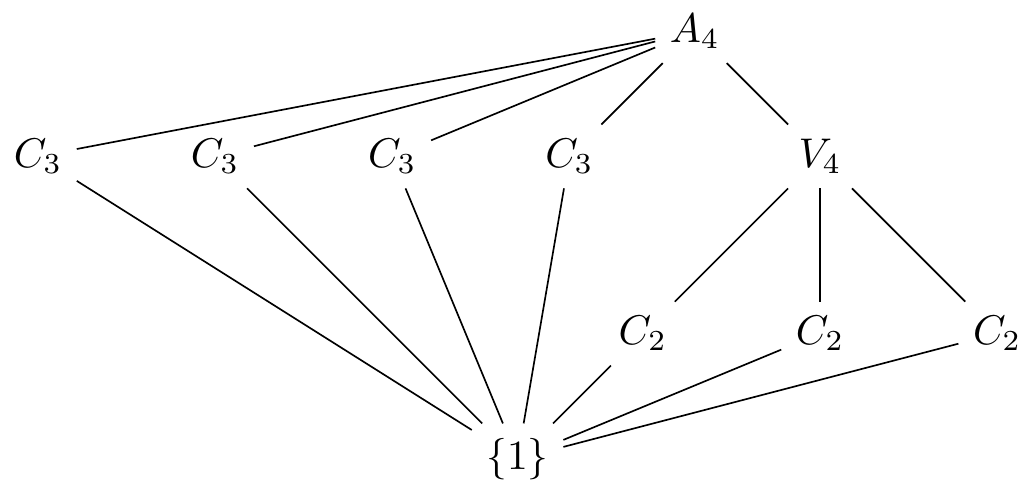
\includegraphics[width=0.5\linewidth]{teoriadegalois_files/figure-latex/unnamed-chunk-1-1}
\end{exercise}

Fent servir l'equació d'un cercle de radi \((x_0,y_0)\) i radi \(r\)
\[
(x-x_0)^2 + (y-y_0)^2 ¡ r^2,
\]
podem veure que les coordenades de la intersecció amb una recta (posem amb equació \(ax+by=c\)) pertanyen al cos
\(\QQ(x_0,y_0,r,a,b,c)\). També podem comprovar-ho pel cas de la intersecció de dos cercles. Resumint si \(\alpha\) és
construcible en \(n\) passos a partir de punts en un cos \(F\), aleshores hi ha una successió de cossos
\[
F=F_0\subseteq F_1\subseteq F_2\subseteq F_n,
\]
amb \([F_{i+1}\colon F_i] \leq 2\), tals que \(\alpha\in F_n\). En particular, \(\alpha\) és un nombre algebraic sobre \(F\) de grau una potència de \(2\).

D'aquí en deduïm directament el següent teorema (on haurem d'assumir que \(\pi\) és transcendent, cosa que no demostrem).

\begin{theorem}
Els tres problemes clàssics no són resolubles.
\end{theorem}

\begin{proof}
Per la duplicació d'un cub de costat \(1\) ens caldria construir \(\sqrt[3]{2}\), que té grau \(3\) i, per tant, no és constructible.

Si un angle \(\theta\) és constructible, aleshores fàcilment veiem que \(\cos(\theta)\) i \(\sin(\theta)\) també són constructibles.
Veurem que \(\alpha=2\cos(\pi/9)\) no és constructible. Com que \(\cos(\pi/3)=1/2\), a partir de la fórmula de l'angle triple obtenim
\[
\alpha^3 - 3\alpha -1 =0.
\]
El polinomi \(x^3-3x-1\) és irreductible (substituint \(x-2\) obtenim un polinomi \(3\)-Eistenstein) i per tant \(\alpha\) té grau \(3\) i
no és constructible.

Finalment, per la quadratura del cercle de radi \(1\) hauríem de construïr un quadrat de costat \(\sqrt{\pi}\). Però aleshores
també podríem construir \(\pi\), que és transcendent (com hem dit, no ho demostrem).
\end{proof}

Més endavant estudiarem quins angles són constructibles. De fet, tenim el següent:

\begin{theorem}
Sigui \(t\) un enter. L'angle de \(t\) graus (no radians!) és constructible si i només si \(t\) és un múltiple de \(3\).
\end{theorem}

\begin{proof}
Hi ha construccions molt antigues del pentàgon regular (\(72^\circ\)), ja que
\[
\cos(72^\circ) = \frac{1}{4} \, \sqrt{5} - \frac{1}{4},
\]
i encara més del triangle equilàter (\(30^\circ\)), ja que \(\cos(30^\circ)=\sqrt{2}/2\). Com que
podem bisectar qualsevol angle, també podem construir \(18^\circ\) i \(15^\circ\). Finalment, com que \(3=18-15\) també podem construir
l'angle de \(3^\circ\). És clar que no podem construir ni \(2^\circ\) ni \(1^\circ\), perquè aleshores podríem construir també qualsevol
múltiple d'aquests i, per tant, podríem construir \(20^\circ\), que ja sabem que no és possible.
\end{proof}

\hypertarget{construccions-amb-regle-marcat-i-compuxe0s}{%
\section{Construccions amb regle marcat i compàs}\label{construccions-amb-regle-marcat-i-compuxe0s}}

Aquí veurem que si el regle té dues marques a una distància qualsevol, aleshores podem trisecar l'angle i duplicar el cub.

TODO.

\hypertarget{normalitat}{%
\chapter{Normalitat}\label{normalitat}}

El cos de descomposició d'un polinomi juga un paper destacat al llarg del curs.
Aquí el definirem, i en demostrarem l'existència i unicitat (llevat d'isomorfisme).
Aprofitarem per definir extensions normals (aquelles que són cos de descomposició d'un conjunt de polinomis).

Com a aplicació, s'introduiran els polinomis i cossos ciclotòmics, i ho lligarem amb la
demostració de l'existència i unicitat de cossos finits de cardinal potència d'un primer.

També veurem les clausures algebraiques, i una construcció (seguint \textcite{artinalgebra} i \textcite{zbigniew}). Això ens permetrà (assumint el teorema fonamental
de l'àlgebra, que demostrarem més endavant) pensar els elements algebraics sobre \(\QQ\) dins dels complexos.

\hypertarget{cossos-de-descomposiciuxf3}{%
\section{Cossos de descomposició}\label{cossos-de-descomposiciuxf3}}

Diem que un polinomi \(f(x)\in F[x]\) \emph{descomposa completament} en una extensió \(K/F\) si es pot escriure com a producte
de polinomis de grau \(1\).

\begin{definition}[cos de descomposició]
Una extensió \(K/F\) és un \emph{cos de descomposició} del polinomi \(f(x)\in F[x]\) si \(f(x)\) descomposa completament a \(K\) i no ho
fa en cap subextensió \(K/K'/F\).
\end{definition}

\begin{theorem}[existència del cos de descomposició]
\protect\hypertarget{thm:existencia-splittingfield}{}\label{thm:existencia-splittingfield}Sigui \(f(x)\in F[x]\). Aleshores existeix un cos de descomposició \(K/F\) de \(f(x)\).
\end{theorem}

\begin{proof}
Fent inducció en el grau d'\(f\), veiem primer que hi ha un cos \(L/F\) on \(f(x)\) descomposa completament. Després podem
prendre per \(K/F\) la intersecció de totes les subextensions \(L/K'/F\) on \(f(x)\) descomposa completament.
\end{proof}

Fixem-nos que cada vegada que adjuntem una arrel d'un polinomi de grau \(n\), aquest polinomi tindrà un cofactor com a molt de grau \(n-1\). Així,
per obtenir un cos de descomposició en el pitjor dels casos haurem de fer una extensió de grau \(n(n-1)(n-2)\cdots 2\cdot 1=n!\).

Podem fer servir la fórmula de les torres per demostrar una versió més forta d'aixecament de morfismes.

\begin{theorem}[teorema d'aixecament d'isomorfismes]
\protect\hypertarget{thm:iso-lifting}{}\label{thm:iso-lifting}Sigui \(K/F\) una extensió finita, i sigui \(L/F\) una extensió. Aleshores:
\[
|\Hom_{F} (K, L)| \leq [K\colon F].
\]
\end{theorem}

\begin{proof}
Farem inducció en el grau \(n=[K\colon F]\). Quan \(n=1\), el resultat és trivial. En general, prenem un element \(\alpha\in K\setminus F\)
i fem servir la fórmula de les torres i \ref{thm:extensio-morfismes}. El cardinal de \(\Hom_F(F(\alpha), L)\)
és igual al nombre d'arrels d'\(\Irr_{\alpha, F}(x)\) a \(L\), que com a molt és \([F(\alpha) \colon F]\).

En tot cas, si \(\tilde\sigma\) és un d'aquests morfismes, com que \([K \colon F(\alpha)]< [K\colon F]\) podem aplicar la hipòtesi
d'inducció i \(\tilde\sigma\) es pot aixecar a com a molt \([K\colon F(\alpha)]\) morfismes a \(L\).
\end{proof}

Revisant la demostració anterior, obtenim els dos següent corol·laris.

\begin{corollary}
\protect\hypertarget{cor:variacio-aixecament-1}{}\label{cor:variacio-aixecament-1}Siguin \(K/F\) i \(L/F\) extensions d'un cos \(F\). Si existeix \(\alpha\in K\) tal que \(\Irr_{\alpha,F}(x)\)
no té cap arrel a \(L\), aleshores no existeix cap \(F\)-morfisme \(K\to L\).
\end{corollary}

\begin{corollary}
\protect\hypertarget{cor:variacio-aixecament-2}{}\label{cor:variacio-aixecament-2}Suposem que tot polinomi irreductible a \(F\) amb una arrel a \(K\) descomposa completament a \(L\). Aleshores
\[
|\Hom_{F} (K, L)| = [K\colon F].
\]
\end{corollary}

\begin{proposition}[unicitat del cos de descomposició]
\protect\hypertarget{prp:unicititat-splittingfield}{}\label{prp:unicititat-splittingfield}Siguin \(K/F\) i \(K'/F\) dos cossos de descomposició de \(f(x)\in F[x]\). Aleshores \(K \cong K'\).
\end{proposition}

\begin{proof}
Prenem \(L = K'\) al Teorema \ref{thm:iso-lifting} i en repetim la demostració. A cada pas,
podem prendre com a \(\alpha\) una arrel de \(f(x)\) i sempre obtindrem arrels a \(K'\) perquè \(f(x)\)
hi trenca completament.
\end{proof}

\begin{example}
Calcularem els cossos de descomposició dels exemples que estem fent servir: \(x^2-2\), \((x^2-2)(x^2-3)\), \(x^3-2\) i de \(x^4+4\), per exemple, ja
que en aquest cas el cos de descomposició és simplement \(\QQ(i)\).
\end{example}

\begin{example}[cossos ciclotòmics]
\protect\hypertarget{exm:cossos-ciclotomics}{}\label{exm:cossos-ciclotomics}Calculem el cos de descomposició del polinomi \(x^n-1\).
Les seves arrels s'anomenen \emph{arrels \(n\)-èssimes de la unitat}. En els complexos
les arrels són els nombres \(e^{\frac{2\pi i}{n}}\), amb \(n=0,\ldots,n-1\).
Per tant \(\CC\) conté el cos de descomposició de \(x^n-1\). En general,
si \(K/\QQ\) és un cos de descomposició de \(x^n-1\), aleshores podem veure que aquestes
formen un grup amb la multiplicació que, de fet, és cíclic. Diem que una arrel de la unitat
\(\zeta_n\) és \emph{primitiva} si és un generador d'aquest grup. Si en fixem una, les altres primitives
són de la forma \(\zeta_n^a\), amb \(a\) coprimer amb \(n\). Hi ha, doncs, \(\varphi(n)\) arrels primitives.

Anomenem *cos ciclotòmic \(n\)-èssim\$ al cos \(\QQ(\zeta_n)\), que és el cos de descomposició de \(x^n-1\):
si adjuntem \(\zeta_n\), automàticament totes les seves potències pertanyen a aquest cos. A l'episodi
\ref{ciclotomics} aprendrem com calcular el grau d'aquest cos, però --a tall d'espòiler-- podem
veure fàcilment que quan \(n=p\) és primer, aleshores
\[
x^p -1 = (x-1)(x^{p-1}+x^{p-1}+\cdots+x+1),
\]
i ja hem vist que el polinomi \(\Phi_p(x)= x^{p-1}+x^{p-1}+\cdots+x+1\) és irreductible. Per tant, tenim
\[
[\QQ(\zeta_p)\colon\QQ]=p-1.
\]
\end{example}

\begin{example}
Calcularem ara el cos de descomposició de \(x^p-2\), on \(p\) és un primer.
Si anomenem \(\alpha\) una arrel d'aquest polinomi,
aleshores les altres arrels són de la forma \(\alpha\zeta\),
on \(\zeta\) és una arrel \(p\)-èssima de la unitat. Podem veure fàcilment
que el cos de descomposició és \(L = \QQ(\sqrt[p]{2}, \zeta_p)\).

Tenim la torre \(L / \QQ(\zeta_p) / \QQ\) i \(L/\QQ(\zeta_p)\) té grau com a molt \(p\),
ja que està generada per \(\sqrt[p]{2}\). Per tant, es té la desigualtat \([L\colon\QQ]\leq p(p-1)\).
Com que \(L\) té subcossos de grau \(p\) i de grau \(p-1\), aquests dos nombres divideixen el grau de l'extensió total i,
com que són coprimers, en deduim que el grau és exactament \(p(p-1)\). Ho podem il·lustrar amb el diagrama següent:
\[
\xymatrix{
  & \QQ(\sqrt[p]{2},\zeta_p) \\
  \QQ(\zeta_p)\ar@{-}^{p}[ur]\ar@{-}^{p-1}[dr] &&\QQ(\sqrt[p]{2})\ar@{-}[ul]_{p-1}\ar@{-}[dl]_{p}\\
  &\QQ
}
\]
\end{example}

\hypertarget{la-clausura-algebraica}{%
\section{La clausura algebraica}\label{la-clausura-algebraica}}

\begin{definition}[clausura algebraica]
\protect\hypertarget{def:clausura-algebraica}{}\label{def:clausura-algebraica}Diem que \(\bar{F}/F\) és una \emph{clausura algebraica} d'\(F\) si \(\bar{F}/F\) és algebraica i tot polinomi \(f(x)\in F[x]\)
descomposa completament a \(\bar{F}\).
\end{definition}

\begin{definition}[algebraicament tancat]
\protect\hypertarget{def:algebraicament-tancat}{}\label{def:algebraicament-tancat}Un cos \(F\) és \emph{algebraicament tancat} si és una clausura algebraica sobre si mateix. És a dir, si tot
polinomi \(f(x)\in F[x]\) té alguna arrel a \(F\).
\end{definition}

Aviat veurem que tot cos té alguna clausura algebraica, i que hi ha cossos algebraicament tancats. Veurem
primer que les clausures algebraiques són algebraicament tancades.

\begin{proposition}
\protect\hypertarget{prp:clausura-tancada}{}\label{prp:clausura-tancada}Sigui \(\bar{F}/F\) una clausura algebraica de \(F\). Aleshores \(\bar{F}\) és algebricament tancat.
\end{proposition}

\begin{proof}
Considerem un polinomi \(f(x)\in \bar{F}[x]\), i considerem l'extensió \(\bar{F}(\alpha)\) obtinguda adjuntant
una arrel de \(f(x)\) a \(\bar{F}\). Aleshores \(\bar{F}(\alpha)/\bar{F}/ F\) és una torre algebraica, i per tant
l'extensió total és algebraica. En particular, \(\alpha\) és algebraic sobre \(F\) i, per tant, \(\alpha \in \bar{F}\),
com volíem demostrar.
\end{proof}

El següent resultat ens permet trobar una clausura algebraica de qualsevol subcos d'un cos algebraicament tancat.

\begin{proposition}
\protect\hypertarget{prp:clausura-tecnica}{}\label{prp:clausura-tecnica}Sigui \(K/F\) una extensió, i suposem que \(K\) és algebraicament tancada. Aleshores la subextensió \(\bar{F}/F\)
formada pels elements de \(K\) que són algebraics sobre \(F\) és una clausura algebraica de \(F\) .
\end{proposition}

\begin{proof}
L'extensió \(\bar{F} / F\) és algebraica per definició. Donat un polinomi
\(f(x)\in F[x]\), aquest trencarà completament a \(K\) en producte de polinomis de la forma \(x-\alpha\). Però
cadascun dels \(\alpha\) és algebraic sobre \(F\) i, per tant, és un element de \(\bar{F}\). Per tant \(f(x)\) ja trencava
completament a \(\bar{F}[x]\), i per tant \(\bar{F}\) és una clausura algebraica de \(F\).
\end{proof}

Cap al final del curs veurem una demostració del següent teorema, que també es pot demostrar amb mètodes analítics.

\begin{theorem}[Teorema Fonamental de l'Àlgebra]
\protect\hypertarget{thm:fta}{}\label{thm:fta}El cos \(\CC\) dels nombres complexos és algebraicament tancat
\end{theorem}

Com a conseqüència, podrem clausures algebraiques de qualsevol extensió subextensió \(\CC/F/\QQ\). En particular,
el cos \(\QQbar\) format pels complexos algebraics és una clausura algebraica de \(\QQ\).

Donat un cos qualsevol \(F\), tenim ara l'objectiu de construir una clausura algebraica \(\bar{F}/F\). Intuitivament almenys,
la idea és de considerar, per cada polinomi \(g(x)\in F[x]\), un cos \(F_g\) que contingui totes les arrels de \(g\).
Aleshores hauríem de prendre el compositum de tots aquests cossos. El problema és que per fer el compositum
hem de prendre una intersecció de molts cossos, i no està clar on viuen aquests cossos (la intersecció
de conjunts només té sentit quan aquests conjunts són subconjunts d'un conjunt fixat). Fixem-nos que si
només consideréssim un nombre finit de polinomis \(g_1(x),\ldots, g_n(x)\) aleshores podríem prendre
el cos de descomposició del producte \(g_1(x)\cdots g_n(x)\).

\begin{theorem}[existència de clausura algebraica]
\protect\hypertarget{thm:existencia-clausura-algebraica}{}\label{thm:existencia-clausura-algebraica}Sigui \(F\) un cos. Aleshores existeix una clausura algebraica \(\bar{F}/F\).
\end{theorem}

\begin{proof}
Considerem un conjunt \(\mathcal{U} \supset F\) de cardinal estrictament superior a \(\mathcal{N}=\max(\aleph_0, |K|)\).

Sigui
\[X = \{K\subseteq L \subseteq S ~|~ L/K \text{ és una extensió algebraica de $K$}\},\]
amb la relació d'ordre
\[
K_2 > K_1 \iff \text{$K_2/K_1$ és una extensió algebraica}.
\]
Com que tota cadena té un element maximal (prenem la unió de totes les extensions), el lema de Zorn
ens diu que hi ha un element maximal a \(X\), que anomenarem \(\bar{F}\). Només ens cal veure que \(\bar{F}/F\) és
una clausura algebraica. Sigui \(f(x)\in F[x]\) un polinomi no constant, i suposem que no té cap zero a \(\bar{F}\).
Podem construir una extensió \(L / \bar{F}\) on \(f(x)\) tingui un zero. Aleshores \(L/F\) és algebraica, i per tant
\[
|\bar{F}| \leq |L| \leq \mathcal{N}.
\]
Per tant, \(|S\smallsetminus \bar{K}| = |S| > |L\smallsetminus \bar{K}|\). Això fa que existeixi
una aplicació (de conjunts) injectiva \(i \colon L \to S\) tal que \(i(x)=x\) si \(x\in \bar{F}\). Podem doncs
transportar l'estructura de cos de \(L\) a \(i(L)\) i obtenim un nou element maximal \(L > \bar{F}\), contradient
la maximalitat de \(\bar{F}\).
\end{proof}

Una demostració alternativa:
::: \{.proof\}
Presentem una demostració alternativa que amaga una mica més els problemes amb la teoria de conjunts. Gràcies
a la Proposició \ref{prp:clausura-tecnica}, n'hi ha prou amb construir una extensió \(K/F\) algebraicament tancada.

Per
cada polinomi mònic no constant \(f=f(x)\in F[x]\), considerem una variable \(x_f\). Tenim l'anell de polinomis
en infinites variables \(F[\{x_f\}]\), i hi podem considerar l'ideal \(I\) generat pels polinomis \(f(x_f)\).

Veurem que \(I\) no és el total i que, per tant, està contingut en un ideal maximal \(\mathcal{M}\). El quocient
l'anomenem \(K_1\), que és una extensió de \(F\) que conté \textbf{una arrel} de cada polinomi amb coeficients a \(F\). Podem
iterar el procés (començant amb \(K_1\) en comptes de amb \(F\)) per obtenir \(K_2/K_1\), una extensió on tot polinomi
amb coeficients a \(K_1\) té una arrel, i així construim una successió de cossos de la qual en podem
prendre la seva ``unió'' \(K\). Donat un polinomi \(f(x)\in K[x]\), tots els seus coeficients viuen necessàriament
a \(K_n\) i, per tant, \(f(x)\) té alguna arrel a \(K_{n+1}\) i, per tant a \(K\).

Ens queda per veure que \(I\) és un ideal propi. Suposem que no i arribarem a contradicció. Suposem que tenim una
relació
\[
g_1 f_1(x_{f_1}) + g_2 f_2(x_{f_2}) + \cdots + g_k f_k(x_{f_k}) = 1,\quad g_i \in F[\{x_f\}].
\]
En total, aquesta relació només involucra un nombre finit de variables. Les hi posem nom: denotem \(x_1=x_{f_1}\),
i així successivament fins a \(x_k = x_{f_k}\). Després anomenem \(x_{k+1},\ldots, x_r\) la resta de variables
que apareixen en els polinomis \(g_i\), de manera que podem reescriure la relació anterior com
\[
g_1(x_1,\ldots, x_r) f_1(x_1) + g_2(x_1,\ldots,x_r) f_2(x_2)+\cdots+g_k(x_1,\ldots x_r) f_k(x_k)=1.
\]
Prenem ara una extensió finita \(F'/F\) que contingui una arrel \(\alpha_i\) de \(f_i(x)\) per cada \(i\). La relació
anterior particularitza, si fem \(x_i=\alpha_i\) per \(i=1,\ldots,k\) i \(x_i=0\) per \(i>k\), a \(0=1\), que és una
contradicció. Això acaba la demostració.
:::

La clausura algebraica és única llevat d'isomorfisme, fet que es pot deduir fàcilment de la unicitat de cossos de descomposició.

\begin{proof}
TODO
\end{proof}

\begin{remark}
L'existència i unicitat de clausures algebraiques fou demostrada per Steinitz el 1910, i la demostració era molt
més llarga i complicada (unes 20 pàgines).

També es pot demostrar (però ens cal teoria que veurem una mica més endavant) que el cos \(K_1\)
que apareix a la demostració anterior ja és algebraicament tancat, així que no caldria fer tots
els altres infinits passos. La demostració d'aquest fet no és senzilla, fa servir el teorema de l'element
primitiu (vegeu \ref{element-primitiu}), i separa els casos de característica \(0\) i característica \(p\).
\end{remark}

\hypertarget{extensions-normals}{%
\section{Extensions normals}\label{extensions-normals}}

\begin{definition}[extensió normal]
\protect\hypertarget{def:ext-normal}{}\label{def:ext-normal}Una extensió algebraica \(K/F\) es diu \emph{normal} si tot polinomi irreductible \(f(x)\in F[x]\) que té una arrel a \(K\) trenca
completament a \(K\).
\end{definition}

Dit d'una altra manera \(K/F\) és normal si per tot \(\alpha\in K\) el seu polinomi mínim sobre \(F\) descomposa completament a \(K\). D'entrada,
sembla difícil demostrar que una extensió donada \(K/F\) és normal, ja que cal veure una propietat per possiblement infinits polinomis. Veurem
ara que les extensions normals tenen una caracterització més senzilla. En particular, el cos de descomposició d'un polinomi
és sempre una extensió normal.

\begin{proposition}
Una extensió \(K/F\) és normal si i només si \(K\) és el cos de descomposició d'un conjunt \(S\subset F[x]\) de polinomis de \(F\).
\end{proposition}

\begin{proof}
Suposem que \(K/F\) és normal. Per cada element \(\alpha\in K\), denotem per \(f_\alpha(x)=\Irr_{\alpha,F}(x)\).
Aleshores \(K\) és el cos de descomposició del conjunt \(S=\{f_\alpha(x)~|~ \alpha\in K\}\).

Recíprocament, si \(K\) és el cos de descomposició d'un conjunt \(S\) i \(f(x)\in F[x]\) té una arrel \(\alpha\in K\),
aleshores sense perdre generalitat podem suposar que \(f(x)\) és irreductible. Considerem el conjunt \(\Sigma\subset K\)
d'elements de \(K\) que són arrels de polinomis a \(S\). Podem trobar un subconjunt finit \(S_0\) i el seu corresponent
conjunt d'arrels \(\Sigma_0\) tals que \(\alpha\in F(\Sigma_0)\). Però aleshores \(F(\Sigma_0)\) és un
cos de descomposició d'un polinomi (el que s'obté multiplicant tots els polinomis de \(S_0\) i extraient-ne la part lliure
de quadrats). Per tant, \(f(x)\) descomposa completament a \(F(\Sigma_0)\) i per tant també a \(K\).
\end{proof}

\begin{proposition}
Sigui \(L/K/F\) una torre. Si \(L/F\) és normal, aleshores \(L/K\) també ho és.
\end{proposition}

\begin{proof}
Trivial: si \(L/F\) és el cos de descomposició d'un conjunt de polinomis \(S\), també ho és del mateix conjunt pensat
com a conjunt de polinomis amb coeficients a \(K\).
\end{proof}

\hypertarget{polinomis-inseparables}{%
\chapter{Polinomis (In)separables}\label{polinomis-inseparables}}

Definim la noció de separabilitat d'un polinomi, i posem algun exemple. Introduïm el morfisme de Frobenius,
que ens permet definir cossos perfectes. Aprofitem per parlar del grau de separabilitat/inseparabilitat d'una
extensió, i la factorització d'aquesta.

Finalment, donem l'existència i unicitat dels cossos finits.

\hypertarget{separabilitat-de-polinomis-i-extensions}{%
\section{Separabilitat de polinomis i extensions}\label{separabilitat-de-polinomis-i-extensions}}

Sigui \(F\) un cos.

\begin{definition}[separabilitat]
\protect\hypertarget{def:separabilitat}{}\label{def:separabilitat}Un polinomi \(f(x)\in F[x]\) és \emph{separable} si les seves arrels (en un cos de descomposició) són totes diferents. Si \(f(x)\)
no és separable diem que \(f(x)\) és \emph{inseparable}.
\end{definition}

Fixem-nos que la definició no depèn del cos de descomposició que ens triem, per unicitat llevat d'isomorfisme. De fet, podem
caracteritzar la separabilitat de \(f(x)\) sense haver de considerar cap cos de descomposició:

\begin{proposition}
\protect\hypertarget{prp:separabilitat-iff-coprimer-derivada}{}\label{prp:separabilitat-iff-coprimer-derivada}Un polinomi \(f(x)\) té una arrel múltiple \(\alpha\) si i només si \(\alpha\) és una arrel de \(f'(x)\). En particular, \(f(x)\)
és separable si i només si \(\mcd(f(x), f'(x)) = 1\).
\end{proposition}

\begin{proof}
TODO (fàcil, fet a fonaments).
\end{proof}

\begin{corollary}
Si \(f(x)\in F[x]\) és irreductible i \(F\) té característica \(0\), aleshores \(f\) és separable. En general,
un polinomi \(f(x)\in F[x]\) és separable si i només si és producte de diferents polinomis irreductibles.
\end{corollary}

\begin{proof}
TODO (molt fàcil).
\end{proof}

\begin{example}
El polinomi \(x^n-1\) té derivada \(nx^{n-1}\) i per tant, si \(n\neq 0\) a \(F\) aleshores \(x^n-1\) és separable, i en aquest cas hi ha \(n\)
arrels de la unitat diferents a \(F\). En canvi, si \(F\) és de característica \(p\mid n\), aleshores cada arrel de \(x^n-1\) és múltiple.
\end{example}

Ja hem estudiat el problema de separabilitat en característica \(0\), que és molt senzill. Ens centrarem ara en característica \(p\), així que
sigui \(F\) un cos de característica finita \(p\). Pensem en què pot anar malament per tal que un polinomi irreductible \(f(x)\in F[x]\) sigui inseparable. Cal que la seva derivada
tingui factors en comú amb \(f(x)\), i això només pot passar si la derivada és \(0\).

\begin{lemma}
Sigui \(f(x)\in F[x]\) amb \(\car(F)=p\). Si \(f'(x)=0\), aleshores hi ha un polinomi \(f_1[x]\in F[x]\) tal que \(f(x)=f_1(x^p)\).
\end{lemma}

En particular, observem que si \(f(x)\in F[x]\) és inseparable, aleshores el seu grau és un múltiple de \(p\).

\begin{proposition}
Sigui \(f(x)\in F[x]\) amb \(\car(F)=p\) un polinomi irreductible. Aleshores hi ha un únic \(k\geq 0\) i un únic
polinomi irreductible i separable \(g(x)\in F[x]\) tal que
\[
f(x)=g(x^{p^k}).
\]
\end{proposition}

\begin{proof}
Iterem el procediment del lema anterior fins que el polinomi que obtenim és separable. Seguirà essent
irreductible, i ja haurem acabat.
\end{proof}

\begin{definition}[grau de separabilitat]
\protect\hypertarget{def:grau-separabilitat}{}\label{def:grau-separabilitat}Sigui \(f(x)\in F[x]\) amb \(\car(F)=p\) un polinomi irreductible. El \emph{grau de separabilitat} de \(f(x)\)
és el grau de \(g(x)\) en la proposició anterior, i el denotem per \(\deg_s f(x)\).

El \emph{grau d'inseparabilitat} és l'enter \(p^k\) que hi apareix, i el denotem per \(\deg_i f(x)\).
\end{definition}

Observem que \(\deg f(x) = \deg_s f(x) \deg_i f(x)\).

\begin{proposition}
\protect\hypertarget{prp:frobenius}{}\label{prp:frobenius}Sigui \(F\) un cos de característica \(p\). Aleshores l'aplicació \(a \mapsto a^p\) és un morfisme de cossos \(F\to F\).
\end{proposition}

\begin{proof}
Només cal veure que \((a+b)^p = a^p + b^p\) i que \((ab)^p = a^p b^p\). La primera igualtat es veu fent servir que \(p\) divideix a \(\binom{p}{i}\)
per a \(1\leq i\leq p-1\), i la segona és trivial.
\end{proof}

El morfisme de la proposició anterior s'anomena el \emph{morfisme de Frobenius}. Observem que si \(\FF\) és un cos finit, aleshores el morfisme de
Frobenius és un isomorfisme (només cal comptar), però en general no és cert.
Per exemple, la imatge de Frobenius a \(F=\FF_p(t)\) és \(\FF_p(t^p)\).

\begin{proposition}
Sigui \(\FF\) és un cos de característica \(p\) tal que el morfisme
de Frobenius és exhaustiu. Aleshores tot polinomi irreductible sobre \(\FF\) és separable.
\end{proposition}

\begin{proof}
Suposem que \(f(x)\) fos inseparable. Aleshores \(f(x)=f_1(x^p)\) per algun \(f_1(x)\in \FF[x]\). Els coeficients de \(f_1\) són potències de \(p\), i
aleshores podem escriure
\[f_1(x)=a_m^px^m+a_{m-1}^px^{m-1}+\cdots a_1^px + a_0^p.\]

Per tant, tenim
\[
f(x)=f_1(x^p) = a_m^px^{pm}+a_{m-1}^px^{p(m-1)}+\cdots a_1^px^p + a_0^p = \left(a_mx^m+a_{m-1}x^{m-1}+\cdots a_1x + a_0\right)^p,
\]
que contradiu el fet que \(f(x)\) sigui irreductible.
\end{proof}

Aquesta definició ens servirà per unificar els dos casos on la separabilitat no és problemàtica.

\begin{definition}[cos perfecte]
\protect\hypertarget{def:cos-perfecte}{}\label{def:cos-perfecte}Un cos \(F\) és \emph{perfecte} si té característica \(0\) o bé el morfisme de Frobenius és exhaustiu.
\end{definition}

\begin{corollary}
Si \(F\) és perfecte, aleshores tot polinomi irreductible a \(F[x]\) és separable.
\end{corollary}

Finalment, podem introduir el concepte d'extensió separable.

\begin{definition}[extensió separable]
\protect\hypertarget{def:ext-separable}{}\label{def:ext-separable}Una extensió \(K/F\) és \emph{separable} si tot element de \(K\) és arrel d'un polinomi separable sobre \(F\).
\end{definition}

\begin{corollary}
Tota extensió finita d'un cos perfecte és separable. En particular, els cossos finits són separables.
\end{corollary}

\begin{corollary}
Sigui \(F\) un cos de característica \(p\), i sigui \(K/F\) una extensió finita tal que \(p \nmid [K\colon F]\).
Aleshores \(K/F\) és separable.
\end{corollary}

\begin{proof}
Sigui \(\alpha \in K\), i considerem \(\Irr_{\alpha, F}(x)\). Com que el seu grau és un divisor de \([K\colon F]\),
no pot ser divisible per \(p\) i, per tant, és separable.
\end{proof}

Més endavant ens serà útil saber que que la separabilitat es comporta bé en torres.
::: \{.lemma\}
Sigui \(L/K/F\) una torre. Si \(L/F\) és separable, aleshores \(L/K\) i \(K/F\) també ho són.
:::
::: \{.proof\}
Si \(L/F\) aleshores \(K/F\) és separable, trivialment. Per veure que \(L/K\) també ho és, observem
simplement que per tot \(\alpha\in L\), el polinomi \(\Irr_{\alpha,K}(x)\) és un divisor (a \(K[x]\)) del polinomi \(\Irr_{\alpha,F}(x)\).
:::

Més endavant veurem que el recíproc també és cert, però per ara no ens caldrà.

\hypertarget{applicaciuxf3-cossos-finits}{%
\section{Applicació : cossos finits}\label{applicaciuxf3-cossos-finits}}

L'objectiu és demostrar l'existència de cossos finits d'ordre qualsevol potència d'un primer, i veure que són únics
(llevat d'isomorfisme).

\begin{theorem}[Existència i unicitat de cossos finits]
Per tot primer \(p\) i tot \(n\geq 1\), hi ha un únic (llevat d'isomorfisme) cos finit d'ordre \(p^n\), que
denotarem per \(\FF_{p^n}\). A més, si \(\FF\) és un cos finit de característica \(p\),
aleshores és isomorf a \(\FF_{p^n}\) per alguna \(n \geq 1\).
\end{theorem}

\begin{proof}
Sigui \(n\geq 1\), i fixem-nos que el polinomi \(f(x)=x^{p^n}-x \in \FF_p[x]\) té derivada \(-1\) i, per tant, és separable.
Si \(\alpha\) i \(\beta\) són dues arrels qualssevol, aleshores \(\alpha\beta\) i \(\alpha+\beta\)
també són arrels. Per tant, el conjunt \(L\) format per les \(p^n\) arrels forma un subcos del cos de
descomposició de \(f(x)\) i, per tant, com que \(L\) conté totes les arrels, ha de ser el propi
cos de descomposició. Com que \(L\) té \(p^n\) elements, té grau \(n\) sobre \(\FF_p\), i per tant hem
vist que hi ha cossos finits de grau \(n\) per qualsevol \(n\geq 1\).

Sigui ara \(\FF\) un cos finit qualsevol de característica \(p\). Com que és un espai vectorial sobre el seu
cos primer \(\FF_p\), ha de tenir \(p^n\) elements per algun \(n\geq 1\). Fixem-nos que \(\FF^\times\) és un grup
d'ordre \(p^n-1\) i, per tant \(\alpha^{p^n-1} = 1\) per tot \(\alpha\in \FF\). Per tant \(\alpha\) és una arrel
de \(x^{p^n}-x\) i \(\FF\) està contingut al cos de descomposició d'aquest polinomi. Mirant el nombre
d'elements, veiem que és igual al cos de descomposició.
\end{proof}

\hypertarget{ciclotomics}{%
\chapter{Polinomis Ciclotòmics}\label{ciclotomics}}

L'objectiu principal és demostrar que l'extensió ciclotòmica \(\QQ(\zeta_n)\) té grau \(\varphi(n)\) (la phi d'Euler). Per això,
introduïrem els polinomis ciclotòmics, veurem que són irreductibles i mònics i tenen coeficients enters.

\hypertarget{definiciuxf3}{%
\section{Definició}\label{definiciuxf3}}

Sigui \(\mu_n\) el grup de les arrels \(n\)-èssimes de la unitat, que podem pensar dins de \(\CC\).
Com a grup abstracte, és isomorf a \(\ZZ/n\ZZ\) (un cop fixem una arrel primitiva \(\zeta_n\)):
\[
\ZZ/n\ZZ \to \mu_n,\quad a \mapsto \zeta_n^a.
\]
Ja hem observat que les arrels primitives són exactament les de la forma \(\zeta_n^a\) amb \(a\) coprimer amb \(n\)
i que, per tant, n'hi ha \(\varphi(n)\). Fixem-nos també que si \(d\mid n\) aleshores \(\mu_d \subseteq \mu_n\).
Però fixem-nos que si \(\zeta\in \mu_n\), aleshores \(\zeta\) és una arrel primitiva \(d\)-èssima per algun \(d \mid n\).

\begin{definition}[polinomi ciclotòmic]
\protect\hypertarget{def:polinomi-ciclotomic}{}\label{def:polinomi-ciclotomic}El \emph{polinomi ciclotòmic \(n\)-èssim} \(\Phi_n(x)\) és el polinomi de grau \(\varphi(n)\) que té per arrels
les arrels primitives de la unitat:
\[
\Phi_n(x) = \prod_{\substack{1\leq a \leq n\\\mcd(a,n)=1}} (x-\zeta_n^a).
\]
\end{definition}

\hypertarget{cuxe0lcul-recursiu}{%
\section{Càlcul recursiu}\label{cuxe0lcul-recursiu}}

Tenim la factorització
\[
x^n - 1= \prod_{\zeta \in \mu_n} (x-\zeta) = \prod_{d\mid n} \Phi_d(x).
\]
En particular, comparant graus tenim la identitat
\[
n = \sum_{d \mid n} \varphi(d).
\]

A més, fixem-nos que la fórmula anterior ens permet calcular els polinomis ciclotòmics de manera recursiva,
dividint pels factors coneguts:
\begin{equation}
\Phi_n(x) = \frac{x^n - 1}{\prod_{\substack{d \mid n\\d < n}} \Phi_d(x)}.
\label{eq:ciclotomics-recursius}
\end{equation}

Els primers valors són, per exemple:

\begin{align*}
\Phi_1(x) &= x-1\\
\Phi_2(x) &= x+1\\
\Phi_{3}(x) &= x^{2} + x + 1 \\
\Phi_{4}(x) &= x^{2} + 1 \\
\Phi_{5}(x) &= x^{4} + x^{3} + x^{2} + x + 1 \\
\Phi_{6}(x) &= x^{2} - x + 1 \\
\Phi_{7}(x) &= x^{6} + x^{5} + x^{4} + x^{3} + x^{2} + x + 1 \\
\Phi_{8}(x) &= x^{4} + 1 \\
\Phi_{9}(x) &= x^{6} + x^{3} + 1 \\
\Phi_{10}(x) &= x^{4} - x^{3} + x^{2} - x + 1 \\
\Phi_{11}(x) &= x^{10} + x^{9} + x^{8} + x^{7} + x^{6} + x^{5} + x^{4} + x^{3} + x^{2} + x + 1 \\
\Phi_{12}(x) &= x^{4} - x^{2} + 1 \\
\Phi_{13}(x) &= x^{12} + x^{11} + x^{10} + x^{9} + x^{8} + x^{7} + x^{6} + x^{5} + x^{4} + x^{3} + x^{2} + x + 1
\end{align*}

\begin{lemma}
Els polinomis \(\Phi_n(x)\) són mònics de grau \(\varphi(n)\) i tenen coeficients enters.
\end{lemma}

\begin{proof}
L'únic que ens cal veure és que \(\Phi_n(x)\) té coeficients enters. Això es veu fàcilment per inducció en \(n\)
i l'algoritme de divisió, fent servir la fórmula \eqref{eq:ciclotomics-recursius}.
\end{proof}

\hypertarget{irreductibilitat}{%
\section{Irreductibilitat}\label{irreductibilitat}}

Amb una mica més de feina podem veure que també són irreductibles.

\begin{theorem}
\protect\hypertarget{thm:ciclotomics-irreductibles}{}\label{thm:ciclotomics-irreductibles}Els polinomis \(\Phi_n(x)\) són irreductibles.
\end{theorem}

\begin{proof}
Prenem \(n\geq 3\), i escrivim una factorització \(\Phi_n(x)=f(x)g(x)\) amb \(f(x)\) i \(g(x)\) mònics a \(\ZZ[x]\), i amb \(f(x)\)
irreductible de grau com a mínim \(2\). L'objectiu és demostrar que \(f(x)=\Phi_n(x)\), és a dir, que tota arrel primitiva \(n\)-èssima
és arrel de \(f(x)\). Sigui doncs \(\zeta\) una arrel \(n\)-èssima primitiva que sigui arrel de \(f(x)\), i veurem
que \(\zeta^a\) també és arrel de \(f(x)\) per a tot \(a\) coprimer amb \(n\).

TODO
\end{proof}

\begin{corollary}
El cos ciclotòmic \(\QQ(\zeta_n)\) té grau \(\varphi(n)\) sobre \(\QQ\).
\end{corollary}

\hypertarget{automorfismes}{%
\chapter{Automorfismes}\label{automorfismes}}

Començarem definint els automorfismes d'una extensió. Veurem que formen
un grup, i que cada subgrup té associat el cos dels elements fixos per aquest. Veurem també
que els automorfismes envien cada element \(\alpha\) a una arrel de \(\Irr(\alpha,x)\),
i demostrarem que en una extensió normal el cardinal del grup d'automorfismes està
fitat pel grau de l'extensió. Així, podrem definir una extensió de Galois com aquella
on la fita s'assoleix.

\hypertarget{definiciuxf3-1}{%
\section{Definició}\label{definiciuxf3-1}}

Sigui \(K\) un cos. Un \emph{automorfisme} de \(K\) és simplement un isomorfisme de \(K\) a \(K\), i el grup d'automorfismes de \(K\) (amb la
composició) s'escriu \(\Aut(K)\).

Si \(\alpha\in K\), diem que \(\sigma\in \Aut(K)\) \emph{fixa} \(\alpha\) si \(\sigma(\alpha)=\alpha\). Més en general,
si \(S\) és un subconjunt de \(K\), diem que \(\sigma\in\Aut(K)\) \emph{fixa} \(S\) si
\(\sigma(x)=x\) per a tot \(x\in S\).

Fixem-nos també que tot automorfisme fixa el cos primer de \(K\) (exercici). En particular, \(\Aut(\QQ)=\Aut(\FF_p)=1\).

Un cas important de subconjunt \(S\) es dona quan tenim una extensió de cossos \(K/F\). En aquest cas,
escrivim \(\Aut(K/F)\) com el grup d'automorfismes que fixen \(F\) (que és un subgrup d'\(\Aut(K)\)):

\[
\Aut(K/F) =\{\sigma \in \Aut(K) ~|~ \sigma(x)=x\,\forall x \in F\}.
\]

\begin{proposition}
Sigui \(K/F\) una extensió, i sigui \(\alpha\in K\) un element algebraic sobre \(F\). Aleshores
per tot \(\sigma\in \Aut(K/F)\) envia \(\alpha\) a una arrel \(\sigma(\alpha)\) de \(\Irr(\alpha,F)(x)\).
\end{proposition}

\begin{proof}
Com que \(\Irr(\alpha,F)(x)\) té coeficients a \(F\) i \(\sigma\) és un morfisme de cossos, tenim
\[
\Irr(\alpha,F)(\sigma(\alpha)) = \sigma(\Irr(\alpha,F)(\alpha)) = \sigma(0)=0.
\]
\end{proof}

\begin{corollary}
Sigui \(f(x)\in F[x]\) un polinomi irreductible i \(K/F\) és una extensió. Aleshores tot automorfisme
\(\sigma\in\Aut(K/F)\) permuta les arrels de \(f(x)\) a \(K\).
\end{corollary}

\begin{corollary}[]
Sigui \(K/F\) una extensió algebraica. Aleshores \(\Hom_F(K, K) = \Aut(K/F)\).
\end{corollary}

\begin{proof}
Sigui \(\sigma \colon K\to K\) un morfisme que fixa \(F\). Ja sabem que és injectiu, però volem veure
que és exhaustiu. Si \(K/F\) és una extensió finita això ja ho sabem (per àlgebra lineal), però aquí
ho volem veure en general. Sigui \(\beta \in K\) qualsevol element. Considerem el conjunt
\[
B = \{\text{arrels de } \Irr_{\beta,F}(x) \text{ a } K \}.
\]
Aleshores \(\sigma\) indueix una aplicació injectiva al conjunt finit \(B\) i, per tant, també exhaustiva. Per tant
hi ha \(\alpha\in B\subseteq K\) tal que \(\sigma(\alpha)=\beta\).
\end{proof}

Aquests resultats ens permeten descriure el grup d'automorfismes d'extensions algebraiques considerant
com actuen aquests automorfismes en els elements que generen l'extensió, ja que tot
automorfisme quedarà únicament determinat per aquesta acció. En particular, quan \(K/F\) és finita
el nombre d'automorfismes també serà finit.

\begin{example}
Calculem \(\Aut(\QQ(\sqrt{2})/\QQ)=\{1,\sigma\}\) i \(\Aut(\QQ(\sqrt[3]{2})/QQ) = 1\).
\end{example}

\hypertarget{cossos-fixos}{%
\section{Cossos fixos}\label{cossos-fixos}}

Fixem \(K\) un cos. Hem vist com associar a cada subcos \(F\subseteq K\) un subgrup \(\Aut(K/F)\) d'\(\Aut(K)\).
Prenem ara la direcció oposada. Associarem a cada subgrup d'automorfismes una certa extensió. Concretament, si
\(S \subseteq \Aut(K)\) és un subconjunt, podem considerar aquells elements de \(K\) que són fixos
per tots els elements de \(S\). És molt fàcil veure que aquest conjunt, que escriurem \(K^S\) i anomenarem
el \emph{cos fix per \(S\)}, és un subcos de \(K\) (exercici). Fixem-nos també que
\[
K^S = K^{\langle S\rangle},
\]
on \(\langle S \rangle\) és el subgrup d'\(\Aut(K)\) generat per \(S\) (el subgrup més petit que conté \(S\)). Per
tant, normalment considerarem només cossos fixos per subgrups d'\(\Aut(K)\) i no perdrem generalitat.

\begin{lemma}
\protect\hypertarget{lem:inc-reversing}{}\label{lem:inc-reversing}Sigui \(K\) un cos.
- Si \(F1\subseteq F_2\subseteq K\), aleshores \(\Aut(K/F_2)\leq \Aut(K/F_1)\).
- Si \(H_1\leq H_2 \leq \Aut(K)\), aleshores \(K^{H_2} \subseteq K^{H_1}\).
\end{lemma}

\begin{proof}
Trivial.
\end{proof}

\begin{lemma}
Sigui \(F\) un cos infinit, i sigui \(V\) un \(F\)-espai vectorial, i siguin \(V_1,\ldots,V_r\) subespais propis.
Aleshores \(V\neq \bigcup V_i\).
\end{lemma}

\begin{proof}
Fem inducció en la dimensió \(n\) de V. El cas \(n=1\) és trivial, així que
podem assumir-ho cert per tot \(F\)-espai vectorial de dimensió \(\leq n-1\) i ho demostrarem per \(V\).
Triem un subespai \(U\subset V\) de dimensió \(n-1\) diferent de tots els \(V_i\) (aquí utilitzem que \(F\) és infinit).
Aleshores apliquem inducció als subespais \(U\cap V_i\) d'\(U\), i obtenim un element d'\(U\) que ja ens serveix.
\end{proof}

\begin{remark}
El lema també és cert quan \(V\) és de dimensió infinita (exercici), però no ens caldrà per les aplicacions.
\end{remark}

\begin{proposition}
\protect\hypertarget{prp:lema-algebra-lineal}{}\label{prp:lema-algebra-lineal}Sigui \(K/F\) una extensió finita, i siguin \(K_1,\ldots,K_r\) subextensions diferents de \(K\). Aleshores hi ha
algun element de \(K\) que no pertany a cap dels \(K_i\).
\end{proposition}

\begin{proof}
Si \(F\) és infinit, ja estem pel lema anterior. Fem doncs el cas on \(F\) és finit. En aquest cas \(K\) també és finit, posem que té \(p^n\) elements. Aleshores
els \(K_i\) també són finits, i tenen \(p^i\) elements cadascun. Com que tots són diferents i hi ha un únic
cos finit de cada cardinal, la unió dels \(K_i\) té com a molt
\[
\sum_{j=0}^{n-1} p^j = \frac{p^n-1}{p-1}
\]
elements, que és menor que \(p^n\).
\end{proof}

\begin{theorem}
\protect\hypertarget{thm:geck}{}\label{thm:geck}Sigui \(K/F\) una extensió finita. Aleshores
\[|\Aut(K/F)| \leq [K\colon F].\]

En particular, \(\Aut(K/F)\) és un grup finit.
\end{theorem}

\begin{proof}
Suposem que \(\Aut(K/F)\) conté \(\sigma_1=1,\ldots,\sigma_{n}\) automorfismes
diferents. Per cada \(i\neq j\), considerem el conjunt
\[
\Eq_{\sigma_i,\sigma_j} = \{x \in K ~|~ \sigma_i(x)=\sigma_j(x)\}.
\]
És fàcil veure que \(\Eq_{\sigma_i,\sigma_j}\subsetneq K\) i que \(\Eq_{\sigma_i,\sigma_j}\) és un cos. Aplicant la proposició anterior,
hi ha algun \(\alpha\in K\) que no està en cap dels \(\Eq_{\sigma_i,\sigma_j}\). El polinomi mínim d'\(\alpha\) sobre \(F\)
té arrels \(\alpha, \sigma_2(\alpha),\ldots,\sigma_{n+1}(\alpha)\), que són totes diferents. Per tant
\([F(\alpha)\colon F]\geq n\). Però \(F(\alpha)\) és una subextensió de \(K\) i, per tant \([K\colon F]\geq n\).
\end{proof}

Donarem un nom doncs a aquelles extensions
que tinguin el nombre màxim d'automorfismes que permet aquesta fita.

\begin{definition}[extensió de Galois]
\protect\hypertarget{def:extensio-galois}{}\label{def:extensio-galois}Sigui \(K/F\) una extensió finita. Diem que \emph{\(K\) és Galois sobre \(F\)} (o que \(K/F\) és una \emph{extensió de Galois})
si \(|\Aut(K/F)| = [K \colon F]\). En aquest cas, escriurem \(\Gal(K/F) = \Aut(K/F)\).
\end{definition}

\begin{corollary}
\protect\hypertarget{cor:fix-gal-eq}{}\label{cor:fix-gal-eq}Sigui \(K/F\) una extensió finita i Galois. Aleshores \(K^{\Gal(K/F)} = F\).
\end{corollary}

\begin{proof}
Escrivim \(G=\Gal(K/F)\), i sigui \(M=K^{G}\supseteq F\). Tenim, per definició, que \(G = \Aut(K/M)\).
Per tant, \([K\colon F] = |G|\leq [K\colon M]\), del que en deduim \(F = M\).
\end{proof}

\begin{corollary}
Sigui \(K/F\) una extensió finita i Galois. Aleshores hi ha un polinomi irreductible i separable
\(f(x)\in F[x]\) de grau \([K\colon F]\) que descomposa completament a \(K\).
\end{corollary}

\begin{proof}
Sigui \(n=[K\colon F]=|\Gal(K/F)|\). A la demostració del teorema, prenem tots els \(n\) automorfismes,
obtenint \(\alpha\in K\) tal que \(F(\alpha) = F\). El seu polinomi mínim \(f(x)\in F[x]\) és irreductible,
de grau \(n\) i té per arrels \(\{\sigma(\alpha) ~|~\sigma\in \Aut(K/F)\}\). Per tant té \(n\) arrels totes diferents,
com volíem.
\end{proof}

Les dues propietats de les extensions de Galois de fet les caracteritzen. Vegem una quarta caracterització
d'aquestes extensions:

\begin{theorem}[Caracterització d'extensions de Galois]
Sigui \(K/F\) una extensió finita i sigui \(G=\Aut(K/F)\). Aleshores els següents enunciats són equivalents:
1. \(|G| = [K\colon F]\).
2. \(F = K^G\).
3. \(K/F\) és normal i separable.
4. Hi ha un polinomi \(f(x)\in F[x]\) irreductible i separable de grau \([K\colon F]\) que descomposa completament a \(K\).
\end{theorem}

\begin{proof}

Ja hem vist \(1 \implies 2\) i \(1 \implies 4\). Fixem-nos també que \(4\implies 3\) és obvi.
- \(2 \implies 3\): Suposem que \(K=F(\alpha_1,\ldots, \alpha_m)\), i considerem el conjunt finit
\[
  B = \{\sigma(\alpha_i) ~|~ \sigma \in G, i = 1,\ldots, m\}.
  \]
Fixem-nos que no sabem quants elements exactament conté \(B\). En tot cas, considerem el polinomi separable
\[
  f(x) = \prod_{\beta \in B} (z - \beta).
  \]
Observem que \(\sigma(f)=f\) per a tot \(\sigma\in G\) i, per tant, \(f \in K^G[x]=F[x]\). Finalment, \(\alpha_i\) és arrel de \(f(x)\)
per a tot \(i=1,\ldots, m\) i concloem que \(K\) és el cos de descomposició de \(f(x)\).

\begin{itemize}
\tightlist
\item
  \(3 \implies 1\): Suposem que \(K/F\) és el cos de descomposició d'un polinomi separable \(f(x)\in F[x]\). Com s'ha
  indicat al Corol·lari \ref{cor:variacio-aixecament-2}, a cada pas podem prendre per \(\alpha\) una arrel del polinomi \(f(x)\)
  i per tant tindrem la igualtat.
\end{itemize}

\end{proof}

\begin{remark}
Suposem que \(K/F\) és de Galois, i sigui \(\alpha\in K\) una arrel del polinomi \(f(x)\) que apareix a la condició \((4)\).
Aleshores \(K=F(\alpha)\). Veiem doncs que tota extensió finita de Galois és primitiva. Més endavant veurem
que només cal que \(K/F\) sigui separable.
\end{remark}

Si \(K/F\) és una extensió de Galois i \(\alpha\in K\), els elements \(\sigma(\alpha)\) (on \(\sigma\in\Gal(K/F)\))
s'anomenen \emph{conjugats de Galois} d'\(\alpha\) sobre \(F\). Si \(K/M/F\) és una subextensió,
el cos \(\sigma(M)\) s'anomena el conjugat de \(M\) per \(\sigma\).

\hypertarget{el-teorema-fonamental}{%
\chapter{El Teorema Fonamental}\label{el-teorema-fonamental}}

Enunciem i demostrem el teorema fonamental de la teoria de Galois. Acabarem
amb diversos exemples concrets d'extensions, il·lustrant la correspondència de Galois.

\hypertarget{preliminars}{%
\section{Preliminars}\label{preliminars}}

\begin{proposition}
Sigui \(K\) una cos qualsevol. Sigui \(G\leq\Aut(K)\) un subgrup finit, i sigui \(F=K^G\). Aleshores \(K\) és Galois sobre \(F\),
i \(\Gal(K/F) = G\).
\end{proposition}

\begin{proof}
Per definició d'\(F\), tenim \(G \leq \Aut(K/F)\), i només ens cal veure la igualtat. El teorema
ens diu que \(|G|=[K\colon F]\), i ja hem vist \(|\Aut(K/F)|\leq [K\colon F]\). Per tant:
\[
[K\colon F] = |G| \leq |\Aut(K/F)| \leq [K\colon F].
\]
Per tant, totes les desigualtats són igualtats i, en particular \(|G| = |\Aut(K/F)|\).
\end{proof}

\begin{corollary}
Si \(G_1\) i \(G_2\) són subgrups diferents d'\(\Aut(K)\), aleshores \(K^{G_1} \neq K^{G_2}\).
\end{corollary}

\begin{proof}
Trivial.
\end{proof}

\hypertarget{la-corresponduxe8ncia-de-galois}{%
\section{La correspondència de Galois}\label{la-corresponduxe8ncia-de-galois}}

Sigui \(K/F\) una extensió finita de Galois. A cada subextensió \(K/M\) li podem associar el seu
grup de Galois, \(\Gal(K/M)\). També podem associar a cada subgrup \(H\leq \Gal(K/F)\) el cos fix \(K^H\).
El següent resultat ens diu que aquestes dues operacions són inverses mútuament.

\begin{theorem}
Sigui \(K/F\) finita Galois. Aleshores \(M\mapsto \Gal(K/M)\) i \(H\mapsto K^H\) estableixen una bijecció
\[
\{\text{ subextensions } K/M/F\} \stackrel{1\colon 1}{\longleftrightarrow} \{\text{ subgrups } H \leq \Gal(K/F)\}.
\]
A més el grau \([M \colon F]\) es correspon amb l'ordre d'\(H\).
\end{theorem}

\begin{proof}
Hem de veure:
1. \(K^{\Gal(K/M)}= M\). Això és automàtic a partir de la proposició i del Corol·lari \ref{cor:fix-gal-eq}.
2. \(\Gal(K / K^H) = H\). Escrivim \(M=K^H\). Ja sabem que \(K/M\) és de Galois, i \(|\Gal(K/M)|= [K\colon M]\).
A més, per definició tenim \(H\leq \Gal(K/M)\). Hem de demostrar la igualtat: donat \(\tau\in \Gal(K/M)\), veurem
que \(K=\bigcup_{\sigma\in H} \Eq(\sigma,\tau)\). Pel Lema \ref{prp:lema-algebra-lineal}, algun dels \(\Eq(\sigma,\tau)\)
ha de ser tot \(K\), i això ens diu que \(\tau\in H\). Per tant, només ens cal comprovar que per tot \(\alpha\in K\),
hi ha algun \(\sigma\in H\) tal que \(\sigma(\alpha)=\tau(\alpha)\). Considerem el polinomi
\[
f(x) = \prod_{\sigma \in H} (x - \sigma(\alpha)) \in K[x].
\]
Fixem-nos que \(\sigma(f)=f\) per tot \(\sigma\in H\) i per tant \(f(x)\in K^H[x] = M[x]\). Com que \(\tau\) fixa \(M\),
tenim que \(\tau(f)=f\). Però aleshores \(\tau(\alpha)\) ha de ser una arrel de \(f\), és a dir, \(\tau(\alpha)=\sigma(\alpha)\)
per algun \(\sigma\in H\), com volíem.
\end{proof}

Hem vist que si \(K/M/F\) és Galois aleshores \(K/M\) també ho és. Què podem dir de l'extensió \(M/F\)?

\begin{proposition}
Sigui \(K/M/F\) una torre amb \(K/F\) Galois, posem \(G=\Gal(K/F)\). Aleshores són equivalents:

\begin{enumerate}
\def\labelenumi{\arabic{enumi}.}
\tightlist
\item
  \(M/F\) és Galois.
\item
  \(H=\Gal(K/M)\) és un subgrup normal de \(G\).
\item
  \(\sigma(M)\subseteq M\) per a tot \(\sigma\in G\).
\end{enumerate}

En aquest cas, \(\Gal(M/F) \cong G / H\).
\end{proposition}

\begin{proof}
Sigui \(H = \Gal(K/M)\).
\(1 \implies 2\): Sigui \(\sigma\in G\). Si \(\alpha\in M\) té polinomi mínim \(f(x)\in F[x]\), aleshores \(\sigma\)
en permuta les seves arrels i, en particular, \$\sigma(\alpha) \in \(M\). Per tant \(\sigma\) restringeix a un
morfisme de \(M\), que ja hem vist que és un automorfisme. Hem construit doncs una aplicació \(G\to H\),
i és fàcil comprovar que és un morfisme de grups. El seu nucli és doncs un subgrup normal, format
per aquells automorfismes \(\sigma\in G\) que fixen \(M\), és a dir, és justament \(\Gal(K/M)\).

\(2 \implies 3\): Sigui \(\sigma \in G\). Per definició, \(\sigma(M) \in K^{\tilde H}\), on \(\tilde H = \sigma H \sigma^{-1}\).
Com que \(H\) és normal \(\tilde H=H\) i \(K^{\tilde H} = K^H = M\).

\(3 \implies 1\): escrivim \(M = F(\alpha_1,\ldots \alpha_n)\), i considerem
\[
B = \{\sigma(\alpha_i) ~|~ \sigma \in G, i=1,\ldots,n\}.
\]
Aleshores \(f(x)=\prod_{\beta in B} (x-\beta)\) és un polinomi separable amb coeficients
a \(F\). La hipòtesi és que \(B\subseteq M\) i, per tant, \(M\) és el cos de descomposició de \(f\).
\end{proof}

\hypertarget{operacions-de-reticle}{%
\section{Operacions de reticle}\label{operacions-de-reticle}}

Per acabar d'entendre bé la correspondència de Galois, relacionem operacions conegudes entre cossos i entre grups.
::: \{.proposition name=``\,``\}
Sigui \(K/F\) Galois amb \(G = \Gal(K/F)\). Sigui \(M_1\) i \(M_2\) dues subextensions, amb \(H_i=\Gal(K/M_i)\). Aleshores:

\begin{enumerate}
\def\labelenumi{\arabic{enumi}.}
\tightlist
\item
  \(\Gal(K/M_1M_2) = H_1 \cap H_2\), i
\item
  \(\Gal(K/(M_1\cap M_2)) = \langle H_1, H_2\rangle\).
  :::
  ::: \{.proof\}
  Directa, per definició.
  :::
\end{enumerate}

Podem resumir tot l'episodi en un sol resultat:

\begin{theorem}[Teorema fonamental de la teoria de Galois]

Sigui \(K/F\) una extensió de Galois finita amb grup de Galois \(G\). Hi ha una bijecció entre
\[
\{\text{subcossos $K/M/F$}\} \stackrel{1\colon 1}{\longleftrightarrow} \{subgrups H \leq G\}
\]
donada per \$M\mapsto \(H = \Gal(K/M)\) i \(H\mapsto M = K^H\) que satisfà:

\begin{enumerate}
\def\labelenumi{\arabic{enumi}.}
\tightlist
\item
  (gira les inclusions) \(M_1 \subseteq M_2\) si i només si \(H_2\leq H_1\).
\item
  (preserva els graus) \([K\colon M] = |H|\) i \([M \colon F] = [G \colon H]\).
\item
  (preserva normalitat) \(M/F\) és Galois si i només si \(H\) és normal en \(G\).
\item
  (gira els reticles) \(M_1M_2 \leftrightarrow H_1\cap H_2\) i \(M_1\cap M_2 \leftrightarrow \langle H_1, H_2\rangle\).
\end{enumerate}

\end{theorem}

\hypertarget{examples}{%
\section{Examples}\label{examples}}

Calculem alguns exemples, com \(\QQ(\sqrt{2}, \sqrt{3})\), el cos de descomposició de \(\sqrt[3]{2}\), \(\QQ(\sqrt{2}+\sqrt{3})\),
o el cos de descomposició de \(\QQ(\sqrt[8]{2}, \zeta_8)\) de \(\sqrt[8]{2}\).

És important adonar-se que no n'hi ha prou en assignar valors
als generadors d'una extensió per definir un automorfisme, ja que hi pot haver relacions amagades entre els
generadors. Per exemple, si \(\theta=\sqrt[8]{2}\), tenim \(\theta^4 = \zeta_8 + \zeta_8^{-1}\) i per tant no totes
les tries
\(\theta\mapsto \theta\zeta_8^i\) i \(\zeta_8\mapsto \theta_8^j\) amb \(j\) senar donen lloc a automorfismes.

\hypertarget{cossos-finits}{%
\chapter{Cossos Finits}\label{cossos-finits}}

Aplicarem el teorema fonamental de la teoria de Galois a l'estudi complet des cossos finits i les
seves extensions. Sabem que per cada potència de primer \(p^n\) hi ha un únic cos amb \(p^n\) elements,
que anomenem \(\FF_{p^n}\).

\hypertarget{grup-de-galois}{%
\section{Grup de Galois}\label{grup-de-galois}}

Ja vam definir \(\FF_{p^n}\) com el cos de descomposició del polinomi \(x^{p^n}-x\in\FF_p[x]\). Per tant,
l'extensió \(\FF_{p^n} / \FF_p\) és de Galois.

\begin{lemma}
El grup \(\Gal(\FF_{p^n}/ \FF_p)\) és cíclic d'ordre \(n\), generat per l'automorfisme de Frobenius
\[
\sigma \colon \FF_{p^n}\to\FF_{p^n},\quad \alpha\mapsto \sigma(\alpha)=\alpha^p.
\]
\end{lemma}

\begin{proof}
Fixem-nos que \(\sigma\) és un automorfisme, perquè és un endomorfisme injectiu d'un grup finit. També tenim
\(\sigma^i(x) = x^{p^i}\), i per tant \(\sigma\) té ordre \(n\) a \(\Gal(\FF_{p^n}/\FF_p)\). Com que l'ordre
d'aquest grup és \(n=[\FF_{p^n}\colon \FF_p]\), obtenim el resultat.
\end{proof}

\hypertarget{subcossos}{%
\section{Subcossos}\label{subcossos}}

El teorema fonamental ens diu que els subcossos de \(\FF_{p^n}\) estan en correspondència amb els subgrups
de \(\Gal(\FF_{p^n}/\FF_p)=\langle\sigma\rangle\). Sabem de teoria de grups que per cada divisor \(d\mid n\)
hi ha exactament un subgrup d'índex \(d\), que és el generat per \(\sigma^{d}\). A més, tots els subgrups
són normals (perquè és un grup abelià). Per tant, tenim:

\begin{proposition}
Si \(d\mid n\), aleshores \(\FF_{p^d}\) és un subcos de \(\FF_{p^n}\). Recíprocament, si
\(\FF\subseteq\FF_{p^n}\) és un subcos, és de Galois, i \(\FF\cong \FF_{p^d}\) amb \(d\mid n\).
\end{proposition}

Vegem una aplicació fàcil d'aquest resultat:
::: \{.corollary\}
El polinomi irreductible \(\Phi_8(x)=x^4+1\in\ZZ[x]\) és reductible mòdul qualsevol primer \(p\).
:::
::: \{.proof\}
Per \(p=2\), tenim \(x^4+1 = (x+1)^4\). Suposem ara \(p\) senar. Com que \(8\mid p^2-1\) (mirem els quadrats senars
mòdul \(8\)), tenim que \(x^8-1=(x^4-1)(x^4+1)\) divideix a \(x^{p^2-1}-1\) a \(\ZZ[x]\). Per tant, \(x^4+1\) divideix
també a \(x^{p^2}-x\). Això vol dir que les arrels de \(x^4+1\) viuen totes a \(\FF_{p^2}\). Però si fos irreductible,
generaria una extensió de grau \(4\), contradicció.
:::

\hypertarget{polinomis-irreductibles}{%
\section{Polinomis irreductibles}\label{polinomis-irreductibles}}

Ja hem vist que tota extensió de Galois és simple. Obtenim,
per tant:

\begin{proposition}
L'extensió \(\FF_{p^n}/\FF_p\) és simple. Equivalentment, per cada \(n\geq 1\)
existeix un polinomi \(f(x)\in \FF_p[x]\) irreductible de grau \(n\).
\end{proposition}

\begin{proposition}
El polinomi \(x^{p^n}-x\) és el producte de tots els polinomis irreductibles
de grau \(d\), per tots els \(d\mid n\).
\end{proposition}

\begin{proof}
Sigui \(f(x)\) un polinomi irreductible de grau \(d\mid n\). Aleshores l'extensió
generada per \(f\) és de grau \(d\) sobre \(\FF_p\) i per tant és \(\FF_{p^d}\). Per tant,
\(f(x)\) és un divisor de \(x^{p^d}-x\), que al seu torn divideix \(x^{p^n}-x\).

Recíprocament, suposem que \(f(x)\) és un factor irreductible de \(x^{p^n}-x\), podem de grau \(d\). Aleshores
l'extensió que genera és un subcos de \(\FF_{p^n}\) i, per tant, té grau \(d\mid n\).
\end{proof}

\begin{corollary}
El nombre de polinomis irreductibles de grau \(n\) a \(\FF_p[x]\) és:
\[
\Psi(n) = \frac{1}{n} \sum_{d \mid n} \mu(d)p^{n/d},
\]
on \(\mu\) és la funció de Möbius.
\end{corollary}

\begin{proof}
Comptant els graus dels polinomis de la proposició anterior, obtenim
\[
p^n = \sum_{d\mid n} d \Psi(d).
\]
El resultat s'obté aplicant la fórmula d'inversió de Möbius.
\end{proof}

La proposició anterior també ens permet de trobar polinomis irreductibles de manera recursiva. D'entrada,
podem dividir pels polinomis irreductibles de graus \(d\mid n\) amb \(d\le n\) per quedar-nos
amb el producte dels polinomis irreductibles de grau \(n\). Ens caldrà factoritzar-los per
obtenir els factors irreductibles.

TODO: explicar l'algoritme de factorització de Berlekamp.

\hypertarget{la-clausura-algebraica-dff_p}{%
\section{\texorpdfstring{La clausura algebraica d'\(\FF_p\)}{La clausura algebraica d'\textbackslash FF\_p}}\label{la-clausura-algebraica-dff_p}}

Ja hem vist que \(\FF_{p^d}\subseteq \FF_{p^n}\) si i només si \(d \mid n\). Per tant, donades dues extensions
d'\(\FF_p\) com ara \(\FF_{p^{n}}\) i \(\FF_{p^m}\), podem pensar-les dins de \(\FF_{p^{nm}}\). Així, podem
prendre la unió de totes elles i obtenir la clausura algebraica de manera explícita:

\begin{proposition}
Tenim
\[
\overline{\FF}_p = \bigcup_{n\geq 1} \FF_{p^n}.
\]
\end{proposition}

\hypertarget{element-primitiu}{%
\chapter{Element Primitiu}\label{element-primitiu}}

El primer objectiu és demostrar el teorema de l'element primitiu. Recordem que una
extensió \(K/F\) és simple si hi ha algun \(\alpha\in K\) tal que \(K=F(\alpha)\).

\begin{theorem}[caracterització d'extensions simples]
\protect\hypertarget{thm:simple-caracteritzacio}{}\label{thm:simple-caracteritzacio}Una extensió \(K/F\) és simple si i només si hi ha finites subextensions \(K/M/F\).
\end{theorem}

\begin{proof}
Suposem que \(K=F(\alpha)F\) és simple, i sigui \(f(x)=\Irr_{\alpha,F}(x)\). Considerem una subextensió \(K/M/F\).
Aleshores \(g(x)=\Irr_{\alpha,M}(x)\) és un divisor de \(f(x)\) pensats a \(K[x]\). Sigui \(M'\subseteq M\) l'extensió generada
sobre \(F\) pels coeficients de \(g(x)\). Com que \(\Irr_{\alpha,M}(x)=\Irr_{\alpha,M'}(x)\), tenim \([K\colon M]=[K \colon M']\)
i per tant \(M=M'\). En conclusió, els subcossos \(M\) estan generats per coeficients dels factors irreductibles
de \(f(x)\) pensat com a polinomi a \(K[x]\) i, per tant, n'hi ha un nombre finit.

Recíprocament, suposem que \(K/F\) té un nombre finit de subcossos. Gràcies a la Proposicó \ref{prp:lema-algebra-lineal},
hi ha algun \(\alpha\in K\) que no pertany a cap dels subcossos de \(K\). Per tant, \(F(\alpha)=K\).
\end{proof}

\hypertarget{el-teorema-de-lelement-primitiu}{%
\section{El teorema de l'element primitiu}\label{el-teorema-de-lelement-primitiu}}

Amb aquesta caracterització i tot el què sabem fins ara podem demostrar fàcilment el teorema de l'element primitiu.

\begin{theorem}[Element Primitiu]
\protect\hypertarget{thm:element-primitiu}{}\label{thm:element-primitiu}Si una extensió \(K/F\) és finita i separable, aleshores existeix \(\gamma\in K\) tal que \(K=F(\gamma)\).
\end{theorem}

\begin{proof}
Sigui \(L/K\) una extensió tal que \(L/F\) sigui Galois. Per exemple, podem prendre el compositum de tots els
cossos de descomposició dels polinomis mínims d'un conjunt de generadors de \(K/F\). Aleshores \(L/F\) és
primitiva i, pel criteri anterior, hi ha un nombre finit de subcossos de \(L\). En particular, hi ha un
nombre finit de subcossos de \(K\) i, un altre cop pel criteri anterior, l'extensió \(K/F\) és primitiva.
\end{proof}

Podem generalitzar una mica aquest teorema:

\begin{theorem}
Suposem que \(K=F(\alpha,\beta)\) i \(\beta\) és separable sobre \(F\).
Aleshores existeix \(\gamma\in K\) tal que \(K=F(\gamma)\).
\end{theorem}

\begin{proof}
Si \(F\) és un cos finit, aleshores \(F(\alpha,\beta)\) també és un cos finit i per tant sabem que és simple. Suposem
doncs que \(F\) és infinit, i escrivim \(f(x)\) i \(g(x)\) pels polinomis mínims d'\(\alpha\) i \(\beta\), respectivament.
Sigui \(L/F(\alpha,\beta)\) un cos de descomposició per \(f(x)g(x)\), i escrivim \(\alpha=\alpha_1, \alpha_2,\ldots \alpha_r\)
per les arrels de \(f(x)\) a \(L\) i \(\beta=\beta_1,\beta_2,\ldots,\beta_s\) per les arrels de \(g(x)\) a \(L\). Per cada \(i\)
i per cada \(j\neq 1\), l'equació
\[
\alpha_i + X \beta_j = \alpha + X \beta_j
\]
només té la solució \(X=\frac{\alpha_i-\alpha}{\beta-\beta_j}\) (el denominador no és zero perquè \(g(x)\) és separable).
Per tant, com que \(F\) és infinit podem prendre \(t\in F\) que no sigui cap de les solucions anteriors, i definim
\(\gamma=\alpha+t\beta\). Veurem que \(F(\alpha,\beta)=F(\gamma)\). N'hi ha prou amb veure que \(\beta\in F(\gamma)\),
perquè aleshores \(\alpha=\gamma-t\beta\) també hi serà. Considerem els polinomis a \(g(x)\) i \(h(x)=f(\gamma - tx)\)
a \(F(\gamma)\). Observem que \(g(\beta)=0\) i \(h(\beta)=f(\gamma-t\beta) = f(\alpha)=0\). Però les altres arrels
de \(g(x)\) són les \(\beta_j\) amb \(j>1\), i \(h(\beta_j)\neq 0\) en aquest cas. Per tant, \(\mcd(g(x),h(x))=(x-\beta)\)
i en deduim que \(\beta\in F(\gamma)\), com volíem.
\end{proof}

\hypertarget{galois-i-compositum-dextensions}{%
\section{Galois i compositum d'extensions}\label{galois-i-compositum-dextensions}}

Estudiem ara com es comporta la propietat de ser Galois quan prenem compositums.

Suposem que tenim extensions \(K/F\) i \(F'/F\).

\begin{proposition}
Si \(K/F\) és de Galois, aleshores \(KF'\) és de Galois sobre \(F'\) i la restricció indueix
un isomorfisme \(\Gal(KF'/F') \cong \Gal(K/K\cap F')\):
\[
\xymatrix{
  & KF'\\
K \ar@{-}[ur]^{G}& & F' \ar@{-}[ul]_{G}\\
& K\cap F'\ar@{-}[ul]\ar@{-}[ur]\\
& F\ar@{-}[u].
}
\]
En particular, si \(F'/F\) és finita, aleshores
\[
[KF': F] = \frac{[K\colon F] [F' \colon F]}{[K\cap F' \colon F]}.
\]
\end{proposition}

\begin{proof}
Sabem que \(K\) és el cos de descomposició d'un polinomi separable \(f(x)\in F[x]\).
Aleshores, \(KF'\) és el cos de descomposició del mateix polinomi \(f(x)\) ara
pensat com a polinomi a \(F'[x]\).
Considerem ara el morfisme restricció
\[
\varphi \colon \Gal(KF'/F') \to \Gal(K/F).
\]
Està ben definit: donat \(\sigma\in\Gal(KF'/F')\), com que \(F\) és
un subcos de \(F'\) també fixa els elements de \(F\), i per tant la seva
restricció a \(K\) dona lloc a un element de \(\Gal(K/F)\). Calcularem
el nucli i la imatge de \(\varphi\).

Si \(\sigma\in\Gal(KF'/F')\), i suposem que \(\sigma|_K=1\), vol dir
que \(\sigma\) fixa \(K\). Com que també fixava \(F'\),
fixa tot \(KF'\) i per tant és la identitat a \(\Gal(KF'/F')\). Així doncs, \(\varphi\)
és injectiva.

Sigui \(H=\operatorname{Im}(\varphi)\leq \Gal(K/F)\) la imatge, i sigui \(M=K^H\) el seu subcos fix.
Volem veure que \(M=K\cap F'\), i això ens donarà el resultat gràcies a la correspondència
de Galois. Si \(\sigma\in H\), aleshores \(\sigma\) fixa \(F'\). Per tant, \(K\cap F'\subseteq M\).
D'altra banda, el compositum \(M F'\) és fix per tot \(\sigma\in \Gal(KF'/F')\), ja que aquest
\(\sigma\) fixa els elements de \(F'\) i en els elements de \(K\) hi actua via la restricció. Pel
teorema fonamental, \(MF'= F'\) i, per tant \(M\subseteq F'\), d'on en traiem \(K \cap F'=M\).

La fórmula final s'obté comptant graus d'extensions.
\end{proof}

\begin{remark}
Considerem \(F=\QQ\), \(K=\QQ(\sqrt[3]{2})\) (el nostre prototipus d'extensió no normal)
i \(F'=\QQ(\zeta_3\sqrt[3]{2})\), on \(\zeta_3\) és una arrel
cúbica primitiva de la unitat. Tenim \([K\colon F]=[F'\colon F]=3\), i \(KF'=\QQ(\zeta_3,\sqrt[3]{2})\) té grau \(6\),
per tant la igualtat no és certa si cap de les extensions inicials és de Galois.
\end{remark}

Estudiem ara el cas on les dues extensions inicials són de Galois.

\begin{proposition}
Siguin \(K_1/F\) i \(K_2/F\) dues extensions de Galois amb grups \(G_1\) i \(G_2\).
Aleshores \(K_1K_2/F\) i \(K_1\cap K_2 /F\) són Galois, i la restricció a \(K_1\) i a \(K_2\)
indueix un isomorfisme
\[
\Gal(K_1K_2 / F) \cong H = \{(\sigma,\tau) \in G_1\times G_2 ~|~ \sigma|_{K_1\cap K_2} = \tau|_{K_1\cap K_2}\}.
\]

En particular, si \(K_1\cap K_2 = F\), aleshores
\[
\Gal(K_1K_2 / F)\cong G_1\times G_2.
\]
\end{proposition}

\begin{proof}
Suposem que \(K_i\) és el cos de descomposició del polinomi separable \(f_i(x)\in F[x]\). Aleshores \(K_1K_2\)
és el cos de descomposició de la part lliure de quadrats de \(f_1(x)f_2(x)\) i per tant \(K_1K_2\) és Galois
sobre \(F\). Sigui ara \(f(x)\) un polinomi irreductible a \(F[x]\) amb una arrel a \(K_1\cap K_2\). Aleshores totes
les arrels de \(f(x)\) són a \(K_1\) i també a \(K_2\) i, per tant, a \(K_1\cap K_2\). Per tant, \(K_1\cap K_2\) és Galois.

Considerem ara l'aplicació
\[
\varphi\colon \Gal(K_1K_2 / F) \to G_1\times G_2,\quad \sigma\mapsto (\sigma|_{K_1}, \sigma|_{K_2}).
\]
És clarament injectiva, i per tant només ens cal estudiar la imatge. Clarament està continguda dins d'\(H\),
i per tant n'hi ha prou amb calcular els ordres. Pel primer teorema d'isomorfisme,
\[
|\operatorname{Im}(\varphi)| = |\Gal(K_1K_2/F)| = [K_1K_2 \colon F].
\]
D'altra banda, fixem-nos que per cada \(\sigma\in \Gal(K_1/F)\) hi ha \(|\Gal(K_2/K_1\cap K_2)|\) elements \(\tau\in \Gal(K_2/K_1\cap K_2)\)
que satisfan \((\sigma,\tau)\in H\). Per tant:
\[
|H| = |G_1| |\Gal(K_2/ K_1\cap K_2)| = |G_1| \frac{|G_2|}{\Gal(K_1\cap K_2 / F)}
\]
i la fórmula de la proposició anterior ens demostra \(|H| = |\operatorname{Im}(\varphi)|\).
\end{proof}

Podem demostrar un cert recíproc:

\begin{proposition}
Suposem que \(K/F\) és una extensió de Galois, i \(G=\Gal(K/F) = G_1\times G_2\). Aleshores \(K\) és el
compositum de dues extensions de Galois \(K_1/F\) i \(K_2/F\) amb \(K_1\cap K_2=F\) i grups de Galois \(G_1\) i \(G_2\), respectivament.
\end{proposition}

\begin{proof}
Definim \(K_1=K^{G_1}\) i \(K_2=K^{G_2}\). Aleshores \(K_1\cap K_2\) correspon a \(\langle G_1,G_2\rangle=G\), per tant
\(K_1\cap K_2=F\). El compositum correspon amb \(G_1\cap G_2=1\), i per tant \(K_1K_2=K\).
\end{proof}

\begin{corollary}[clausura de Galois]
Sigui \(K/F\) una extensió finita separable. Aleshores hi ha una extensió \(E/K/F\) tal que \(E/F\) és Galois\$,
i és mínima en el sentit que si \(E'/K\) és una extensió amb \(E'/F\) Galois, tenim \(E \subseteq E'\). Aquesta
extensió s'anomena la \emph{clausura de Galois} de \(K/F\).
\end{corollary}

\begin{proof}
Ja sabem que hi ha extensions de \(K\) que són Galois (prenem el cos de descomposició dels polinomis mínims
d'un conjunt de generadors de \(K\)). El cos \(E\) buscat és llavors la intersecció de totes les extensions \(E'/K\) tals
que \(E'/F\) és Galois. Hem vist que aquesta intersecció serà Galois.
\end{proof}

\hypertarget{extensions-abelianes-i-ciclotuxf2miques}{%
\chapter{Extensions Abelianes i ciclotòmiques}\label{extensions-abelianes-i-ciclotuxf2miques}}

En aquest apartat estudiem les extensions ciclotòmiques, i veiem que \(\Gal(\QQ(\zeta_n)/\QQ)\)
és canònicament isomorf a \((\ZZ/n\ZZ)^\times\). Com a aplicació, veurem com construir
polígons regulars amb regle i compàs. Veurem que només és possible per polígons regulars
de \(n\) costats quan \(\varphi{n}\) és una potència de \(2\). Això passa si i només si \(n\) és producte
d'una potència de dos i de primers de Fermat diferents.

\hypertarget{grup-de-galois-dels-cossos-ciclotuxf2mics}{%
\section{Grup de Galois dels cossos ciclotòmics}\label{grup-de-galois-dels-cossos-ciclotuxf2mics}}

Sigui \(n\geq 2\) i considerem el cos ciclotòmic \(\QQ(\zeta_n)\). Volem estudiar \(\Gal(\QQ(\zeta_n)/\QQ)\).
Per cada \(a\in\ZZ\) coprimer amb \(n\), definim l'aplicació
\[
\sigma_a \colon \QQ(\zeta_n)\to \QQ(\zeta_n),\quad \zeta_n\mapsto \zeta_n^a.
\]

\begin{theorem}
L'aplicació \(a \mapsto \sigma_a\) indueix un isomorfisme
\[
\psi \colon (\ZZ/n\ZZ)^\times \to \Gal(\QQ(\zeta_n)/\QQ).
\]
\end{theorem}

\begin{proof}
Ja sabem que \(\Gal(\QQ(\zeta_n)/\QQ)\) té exactament \(\varphi(n)\) elements. Si \(\sigma\) és un
d'aquests automorfismes, sabem que ve determinat per on envia \(\zeta_n\), que és una arrel
del polinomi ciclotòmic \(\Phi_n(x)\). Per tant, \(\sigma(\zeta_n)\) és una arrel \(n\)-èssima primitiva
de la unitat i doncs ha de ser \(\zeta_n^a\) per alguna \(a\) coprimera amb \(n\). Així veiem que
\(\sigma_a\in \Gal(\QQ(\zeta_n)/\QQ)\) i \(\psi\) és una aplicació ben definida i a més exhaustiva, per
tant bijectiva. A més, \(\psi\) és un morfisme de grups, ja que
\[
(\sigma_a\sigma_b)(\zeta_n) = \sigma_a(\zeta_n^b) = (\zeta_n^b)^a = \zeta_n^{ab} = \sigma_{ab}(\zeta_n).
\]
\end{proof}

Fixem-nos que en particular tenim exemples d'extensions cícliques de grau \(p-1\) per qualsevol primer \(p\).
També tenim una versió més conceptual del teorema xinès dels residus, que escrivim en el cas de dos factors
per estalviar notació.

\begin{proposition}
Si \(n\) i \(m\) són coprimers, aleshores \(\QQ(\zeta_n) \cap \QQ(\zeta_m) = \QQ\), \(\QQ(\zeta_n,\zeta_m) = \QQ(\zeta_{nm})\), i
\[
\Gal(\QQ(\zeta_{nm})/\QQ) \cong \Gal(\QQ(\zeta_n)/\QQ) \times \Gal(\QQ(\zeta_m)/\QQ).
\]
\end{proposition}

\begin{proof}
TODO
\end{proof}

El següent lema ens permet trobar generadors dels subcossos de \(\QQ(\zeta_p)\).

\begin{lemma}
Sigui \(p\) un primer, i sigui \(H\leq \Gal(\QQ(\zeta_p)/\QQ)\) un subgrup. Aleshores
\[
\theta_H=\sum_{\sigma \in H} \sigma(\zeta_p)
\]
és un generador del cos fix d'\(H\). L'element \(\theta_H\) s'anomena un \emph{període} de \(\zeta_p\).
\end{lemma}

\begin{example}
Calcularem el reticle de subcossos de \(\QQ(\zeta_{13})\), fent servir el lema anterior.
TODO
\end{example}

\hypertarget{extensions-abelianes}{%
\section{Extensions abelianes}\label{extensions-abelianes}}

Podem fer servir el què hem vist per demostrar el següent resultat.

\begin{theorem}[realització de grups abelians]
Sigui \(G\) un grup finit abelià. Aleshores hi ha una extensió \(K/\QQ\) continguda dins d'un cos ciclotòmic
tal que \(\Gal(K/\QQ) \cong G\).
\end{theorem}

\begin{proof}
Tot grup abelià és producte de cíclics:
\[
G \cong C_{n_1}\times C_{n_2}\times\cdots\times C_{n_k}.
\]
Existeixen primers diferents \(p_1\), \(p_2\), \ldots \(p_k\) tals que \(p_i\equiv 1\pmod{n_i}\). Aquest fet
es dedueix del fet que hi ha infinits primers \(\equiv 1\pmod{m}\) per qualsevol \(m\) (TODO).

Considerem \(n=p_1p_2\cdots p_k\). Aleshores, tenim
\[
\Gal(\QQ(\zeta_n)/\QQ)\cong (\ZZ/(p_1-1))^\times \times (\ZZ/(p_2-1))^\times \times \cdots \times (\ZZ/(p_k-1))^\times.
\]
Com que \(n_i\) divideix \(p_i-1\), hi ha un subgrup \(H_i\leq C_{p_i-1}\) d'índex \(n_i\) per cada \(i\), i el quocient
per \(H_1\times H_2\times\cdots\times H_k\) és isomorf a \(G\). Per la correspondència de Galois, hi ha un subcos
de \(\QQ(\zeta_n)\) que realitza \(G\).
\end{proof}

Els cossos ciclotòmics són exemples d'extensions de Galois amb grup abelià. En general, una
extensió \(K/F\) es diu que té la propietat \(P\) si és de Galois i el seu grup de Galois té la propietat \(P\).
Per exemple, tenim la següent definició:

\begin{definition}[extensió abeliana]
Una extensió \(K/F\) és \emph{abeliana} si \(K/F\) és de Galois i \(\Gal(K/F)\) és un grup abelià.
\end{definition}

El resultat anterior té un recíproc que no podem demostrar aquí:

\begin{theorem}[Kronecker-Weber]
Sigui \(K/\QQ\) una extensió finita abeliana. Aleshores \(K\) està contingut en una extensió ciclotòmica.
\end{theorem}

En general, és avui un problema obert el determinar quins grups apareixen quan com a grups de Galois d'extensions
\(K/\QQ\). Ja hem vist que tots els grups abelians apareixen, però hi ha grups (per exemple \(\PSL_2(\FF_{125})\)) pels
quals no s'ha demostrat encara que hi apareguin. Aquest problema s'anomena el \textbf{problema invers de la teoria de Galois}.

\hypertarget{constructibilitat-de-poluxedgons-regulars}{%
\section{Constructibilitat de polígons regulars}\label{constructibilitat-de-poluxedgons-regulars}}

Com a aplicació dels cossos ciclotòmics, estudiarem quins polígons regulars es poden construir amb regle i compàs.
Ja hem vist que un nombre real \(\alpha\) és construible si i només si \(\QQ(\alpha)\) està contingut en un cos \(K\)
obtingut a partir de \(\QQ\) a partir d'un nombre finit d'extensions quadràtiques.

Construir un polígon de \(n\) costats és equivalent a construir les arrels \(n\)-èssimes de la unitat \(\zeta_n\), que al
seu torn és equivalent a construir la seva part real \(x=\frac{1}{2}(\zeta_n+\zeta_n^{-1})\). Com que
\(\zeta_n^2 - 2 x \zeta_n + 1=0\), el cos \(\QQ(zeta_n)\) és una extensió de grau \(2\) sobre \(\QQ(x)\) (aquesta última és real,
mentre que \(\QQ(\zeta_n)\) no). Per tant, si volem que el cos \(\QQ(x)\) estigui dins de \(K\) ens cal en particular que
el seu ordre \(\varphi(n)/2\) sigui potència de \(2\), és a dir, que \(\varphi(n)\) sigui potència de \(2\).

Recíprocament, si \(\varphi(n)\) és una potència de \(2\), aleshores \(\QQ(x)\) té ordre una potència de \(2\). Prenent
successivament subgrups d'índex \(2\) i fent servir la correspondència de Galois, obtenim una successió
\[
\QQ = K_0 \subset K_1\subset\cdots\subset K_m = \QQ(x),\quad [K_i \colon K_{i-1}] = 2,
\]
i per tant \(x\) és constructible. D'aquí tenim la següent caracterització. Recordem que un primer \(p\) es
diu \emph{primer de Fermat} si \(p-1\) és una potència de \(2\).

\begin{theorem}[construcció de polígons regulars]
Sigui \(n\) un enter positiu. Aleshores el polígon regular de \(n\) costats és constructible
amb regle i compàs si i només si \(n\) és de la forma
\[
n = 2^k p_1 \cdots p_r,
\]
on \(k\geq 0\) i \(p_i\) són primers de Fermat diferents.
\end{theorem}

\begin{proof}
Escrivim \(n\) com a producte de potències de primers diferents
\[
n=2^{k}q_1^{e_1} q_2^{e_2}\cdots q_r^{e_r}, \quad q_i \text{ senar.}
\]
Aleshores tenim la fórmula coneguda
\[
\varphi(n) = 2^{k-1} \prod_{i=1}^r (q_i-1)q_i^{e_i-1}.
\]
Ja veiem que cal que \(e_i=1\) per tot \(i\) si volem que \(\varphi(n)\) sigui potència de \(2\). A més, cal
que \(q_i-1\) sigui potència de \(2\) per a tot \(i\), és a dir que \(q_i\) sigui un primer de Fermat.
\end{proof}

Només es coneixen cinc primers de Fermat: \(F_0=3\), \(F_1=5\), \(F_2=17\), \(F_3=257\), \(F_4=65537\). En general,
si \(p\) és un primer de Fermat aleshores \(p=2^{2^i}+1\) per algun \(i\geq 0\). Els nombres \(F_i=2^{2^i} +1\) s'anomenen
\emph{nombres de Fermat}. Sembla poc probable que hi hagi infinits primers de Fermat, però és encara un problema obert.

La següent expressió dona (en principi) una manera de construir un \(17\)-gon regular amb regle i compàs.
\[
\cos\frac{2\pi}{17} = \frac{1}{16}\left(\sqrt{17}-1+\sqrt{34-2\sqrt{17}}\right)+ \frac{1}{8}\left(\sqrt{17+3\sqrt{17}-\sqrt{34-2\sqrt{17}}-2\sqrt{34+2\sqrt{17}}} \right).
\]

\hypertarget{grups-de-polinomis}{%
\chapter{Grups de Polinomis}\label{grups-de-polinomis}}

En aquest episodi estudiem els grups de Galois de polinomis separables.

\begin{definition}[grup de Galois d'un polinomi]
Sigui \(f(x)\in F[x]\) un polinomi separable amb coeficients a un cos \(F\). El \emph{grup de Galois d'\(f(x)\)}
és el grup de Galois del cos de descomposició de \(f(x)\), que escriurem \(\Gal(f)\).
\end{definition}

Sigui \(K/F\) una extensió de Galois. Aleshores \(K\) és el cos de descomposició d'un polinomi separable \(f(x)\in F[x]\).
Com que les arrels de \(f(x)\) generen \(K/F\), tot element de \(\Gal(K/F)\) ve determinat per on envia cadascuna
de les arrels de \(f(x)\), que necessàriament és una altra arrel. Així, si etiquetem les arrels de \(f(x)\) com
\(\alpha_1,\ldots,\alpha_n\), obtenim un morfisme de grups injectiu
\[
\Gal(K/F)\injects S_n,
\]
que ens permet pensar \(\Gal(K/F)\) com un subgrup de \(S_n\). De fet, si \(f(x)\) no és irreductible i factoritza com
\[
f(x) = f_1(x)\cdots f_k(x),
\]
possiblement amb repetició, i \(\deg(f_i(x)) = n_i\), aleshores
\[
\Gal(K/F)\injects S_{n_1}\times \cdots S_{n_k},
\]
ja que els elements de \(\Gal(K/F)\) permuten les arrels de cadascun dels \(f_i(x)\) per separat.

\begin{remark}[]
Suposem que \(f(x)\) és irreductible. Aleshores el subgrup de \(G\leq S_n\) que obtenim com a imatge de \(\Gal(K/F)\) és \emph{transitiu}: donats \(i,j\),
hi ha un element \(g\in G\) tal que \(g(i)=j\). Així, no tots els subgrups de \(S_n\) són possibles grups de Galois.
\end{remark}

\begin{example}
Calculem els grups de Galois \(\Gal(\QQ(\sqrt{2}, \sqrt{3}) / \QQ)\) i \(\Gal(\QQ(\sqrt[3]{2})/\QQ)\) com a
subgrups de \(S_4\) i \(S_3\), respectivament.
\end{example}

\hypertarget{el-grup-de-galois-del-polinomi-genuxe8ric}{%
\section{El grup de Galois del polinomi genèric}\label{el-grup-de-galois-del-polinomi-genuxe8ric}}

Fixem un cos \(F\), i considerem el cos \(F(s_1,\ldots,s_n)\), on \(s_i\) són indeterminades. Els elements
d'aquest cos són quocients de polinomis en les variables \(s_i\) (s'anomenen funcions racionals).
Considerem el polinomi
\[
f(x) = x^n-s_1x^{n-1} + s_2x^{n-2} + \cdots + (-1)^n s_n \in F(s_1,\ldots, x_n),
\]
que té arrels \(x_1,\ldots,x_n\) que satisfan
\begin{align*}
s_1&=x_1+x_2+\cdots+x_n\\
s_2&=x_1x_2 + x_1x_3 + \cdots x_{n-1}x_n\\
&\cdots\\
s_n&=x_1x_2\cdots x_n.
\end{align*}
El polinomi \(f(x)\) s'anomena el \emph{polinomi general de grau \(n\)}.

\begin{theorem}
El polinomi general de grau \(n\) és separable sobre \(F(s_1,\ldots,s_n)\),
amb grup de Galois \(S_n\).
\end{theorem}

\begin{proof}
El cos de descomposició del polinomi general de grau \(n\) \(f(x)\) és justament
\(F(x_1,\ldots,x_n)\). Suposem que \(p(t_1,\ldots,t_n)\) fos un polinomi en \(n\) variables
i coeficients a \(F\) tal que \(p(x_1,\ldots,x_n)=0\). Aleshores podem prendre el producte
de \(p(x_{\sigma(1)}, x_{\sigma(2)}, \ldots,x_{\sigma(n)})\) amb \(\sigma\) variant per tot
\(S_n\), i obtenim un polinomi simètric \(\tilde p\) tal que \(\tilde p(x_1,\ldots,x_n)=0\).
Però això donaria una relació no trivial entre \(s_1,\ldots,s_n\), contradicció.
\end{proof}

Aquest resultat es pot interpretar com que un polinomi ``genèric'' de grau \(n\) tindrà grup de Galois \(S_n\).
Tot i així, cal anar amb compte amb el significat de ``genèric'': per exemple, els grups de Galois d'un
polinomi irreductible sobre un cos finit sempre és cíclic, així que no serà \(S_n\) si \(n > 3\). Sí que és
cert però que la ``majoria'' de polinomis sobre \(\QQ\) tenen grup de Galois \(S_n\) (en un cert sentit de ``majoria'').

\begin{definition}[discriminant]
\protect\hypertarget{def:discriminant}{}\label{def:discriminant}El \emph{discriminant} d'un polinomi de grau \(n\) amb arrels \(x_1,\ldots,x_n\) és
\[
\disc(f(x)) = \prod_{i < j} (x_i-x_j)^2.
\]
\end{definition}

Com que el discriminant és un polinomi simètric en les arrels de \(f(x)\), es pot expressar
en termes dels seus coeficients. En particular, el discrimiant del polinomi general és un
element \(D\in F(s_1,\ldots,s_n)\).

\begin{theorem}
Sigui \(f(x)\in F[x]\). Aleshores \(\Gal(f)\) és un subgrup del grup alternat \(A_n\) si i
només si \(\disc(f(x))\) és el quadrat d'un element de \(F\).
\end{theorem}

\begin{proof}
Siguin \(x_1,\ldots,x_n\) les arrels de \(f(x)\), i sigui \(D=\disc(f(x))\). Aleshores \(\sqrt{D}=\prod_{i < j} (x_i - x_j)\)
és un element del cos de descomposició de \(f(x)\). Un element \(\sigma\in S_n\) té signe parell
si i només si preserva \(\sqrt{D}\) (per definició del signe). Per tant, \(\sqrt{D}\) és un element de \(F\)
si i només si tot element de \(\Gal(f)\) té signe parell, si i només si \(\Gal(f)\) és un subgrup d'\(A_n\).
\end{proof}

\hypertarget{el-teorema-fonamental-de-luxe0lgebra}{%
\section{El teorema fonamental de l'àlgebra}\label{el-teorema-fonamental-de-luxe0lgebra}}

Demostrarem que \(\CC=\RR(i)\) és algebraicament tancat, fent servir aquest fet bàsic sobre \(\RR\), que
es demostra amb el teorema del valor mig:

\begin{proposition}
\protect\hypertarget{prp:arrels-real-senar}{}\label{prp:arrels-real-senar}No hi ha cap extensió de \(\RR\) finita de grau senar \(>1\).
\end{proposition}

\begin{proof}
És equivalent a veure que tot polinomi de grau senar amb coeficients reals té una arrel real.
\end{proof}

\begin{lemma}
\protect\hypertarget{lem:no-quadratic-complex}{}\label{lem:no-quadratic-complex}No hi ha cap extensió de grau \(2\) de \(\CC\).
\end{lemma}

\begin{proof}
Hem de veure que l'arrel quadrada d'un nombre complex també és complex. Això és un exercici senzill. Per
exemple, si \(\alpha=a+bi\), aleshores una arrel quadrada és de la forma
\[
\sqrt{\frac{a + \sqrt{a^2+b^2}}{2}} \pm i\sqrt{\frac{-a+\sqrt{a^2+b^2}}{2}}.
\]
\end{proof}

\begin{theorem}[Teorema Fonamental de l'Àlgebra]
Sigui \(K/\RR\) una extensió finita. Aleshores \([K \colon \RR] \leq 2\).
\end{theorem}

\begin{proof}
Podem suposar (prenent la clausura de Galois) que \(K/\RR\) és finita Galois.
Sigui \(G=\Gal(K/\RR)\), i sigui \(H\leq G\) un subgrup
de \(2\)-Sylow. Pel TFTG, el grau \([K^H\colon \RR]\) és senar. Per tant, \(K^H=\RR\) i
això vol dir que \(H=G\), és a dir, que \(G\) és un \(2\)-grup (té ordre una potència de \(2\)).

Suposem doncs que \(|G|\geq 4\), i arribarem a una contradicció. En aquest cas, hi ha subgrups \(H_2\leq H_1\leq G\)
amb \([G\colon H_i] = 2^i\). En termes de cossos fixos, hi ha una extensió de grau \(2\) de \(K^{H_1}=\CC\), que
contradiu el lema anterior.
\end{proof}

\hypertarget{arrels-i-radicals}{%
\chapter{Arrels i radicals}\label{arrels-i-radicals}}

Definirem què vol dir que un polinomi sigui resoluble per radicals, i veurem
que és equivalent a què el seu grup de Galois sigui resoluble. D'aquí en podrem
deduir que els polinomis generals de grau \(\geq 5\) no són resolubles per radicals i,
per tant, no existeix una fórmula que expressi les arrels d'un polinomi en termes
dels seus coeficients. També es mostrarà un exemple concret d'un polinomi de grau \(5\) sobre \(\QQ\)
amb grup de Galois \(S_5\).

\hypertarget{caruxe0cters}{%
\section{Caràcters}\label{caruxe0cters}}

En aquesta secció demostrarem un resultat d'àlgebra lineal que ens caldrà més endavant.

\begin{definition}
\protect\hypertarget{def:caracter}{}\label{def:caracter}Un \emph{caràcter} \(\chi\) d'un grup \(G\) amb valors en un cos \(L\) és un morfisme de grups
\[
\chi \colon G \to L^\times.
\]
\end{definition}

Podem pensar un caràcter \(\chi\) com una funció \(G\to L\).
Les funcions de \(G\) a \(L\) formen un \(L\)-espai vectorial, de manera òbvia.
El següent resultat és degut a Dedekind.

\begin{theorem}[Independència lineal dels caràcters]
\protect\hypertarget{thm:caracters-li}{}\label{thm:caracters-li}Siguin \(\chi_1,\ldots,\chi_n\) caràcters de \(G\) diferents. Aleshores són linealment independents, és a dir, no hi ha
cap combinació lineal no trivial \(a_1\chi_1+\cdots+a_n\chi_n\) que doni lloc a la funció idènticament zero.
\end{theorem}

\begin{proof}
Suposem (reordenant, si cal) que podem escriure
\[
a_1\chi_1 + \cdots a_m\chi_m = 0,
\]
amb tots els \(a_i\neq 0\) (observem \(m\leq n\)) i amb \(m\) mínim. Obtindrem una relació de dependència amb menys termes, arribant així a contradicció.

Prenem \(g_0\in G\) tal que \(\chi_1(g_0)\neq \chi_m(g_0)\). Aleshores tenim
\[
a_1\chi_1(g) + \cdots a_m\chi_m(g) = 0,
\]
i
\[
a_1\chi_1(g_0g) + \cdots a_m\chi_m(g_0g) = 0.
\]
Multiplicant la primera equació per \(\chi_m(g_0)\) i restant-li la segona obtenim, per a tot \(g\),
\[
a_1(\chi_m(g_0)-\chi_1(g_0)) \chi_1(g) + \cdots a_{m-1}(\chi_m(g_0)- \chi_{m-1}(g_0)) \chi_{m-1}(g) = 0.
\]
Com que el primer coeficient és diferent de zero, tenim una relació no trivial amb \(m-1\) termes, contradicció.
\end{proof}

Un cas particular que ens interessa aquí prové de considerar un morfisme no trivial de cossos \(\sigma\colon K\to L\),
que indueix un morfisme de grups entre les unitats \(\sigma\colon K^\times \to L^\times\) (aquesta restricció ja conté
tota la informació que ens cal de \(\sigma\), perquè ja sabem que \(\sigma(0)=0\)). Aleshores \(\sigma\) esdevé un caràcter
del grup \(G=K^\times\), i per tant tenim el següent:

\begin{corollary}
\protect\hypertarget{cor:automorfismes-li}{}\label{cor:automorfismes-li}Si \(\sigma_1,\ldots,\sigma_n\) són morfismes diferents de \(K\) a \(L\), aleshores són linealment independents com a funcions de \(K\).
\end{corollary}

\hypertarget{extensions-cuxedcliques}{%
\section{Extensions cícliques}\label{extensions-cuxedcliques}}

\begin{definition}[extensió cíclica]
\protect\hypertarget{def:ext-ciclica}{}\label{def:ext-ciclica}Una extensió \(K/F\) és \emph{cíclica} si és Galois amb grup de galois cíclic.
\end{definition}

Escriurem \(\mu_n\) pel grup de les arrels \(n\)-èssimes de la unitat (en una clausura algebraica),
i també escriurem \(\sqrt[n]{a}\) per una arrel del polinomi \(x^n-a\).

\begin{proposition}
Sigui \(F\) és un cos de característica no divisora de \(n\) que conté \(\mu_n\). Aleshores si \(a\in F\) l'extensió \(F(\sqrt[n]{a})\)
és cíclica de grau un divisor de \(n\).
\end{proposition}

\begin{proof}
Escrivim \(K=F(\sqrt[n]{a})\). Com que \(\mu_n\subseteq F\), \(K\) és el cos de descomposició de \(x^n-a\) i per tant
és Galois. Sigui \(\alpha=\sqrt[n]{a}\) una arrel fixada. Aleshores tot \(\sigma\in\Gal(K/F)\) porta \(\alpha\) a \(\alpha\zeta_\sigma\),
on \(\zeta_\sigma\in\mu_n\) és una arrel \(n\)-èssima de la unitat que depèn de \(\sigma\). Obtenim així una aplicació
\[
\chi_a\colon \Gal(K/F)\to \mu_n,\quad \sigma\mapsto \zeta_\sigma=\frac{\sigma(\alpha)}{\alpha}.
\]
Fixem-nos que \(\chi_a\) no depèn de quina arrel \(\alpha\) hem triat de \(x^n-a\). Qualsevol altra arrel seria de la
forma \(\alpha\zeta\), i \(\sigma(\alpha\zeta)/(\alpha\zeta) = \sigma(\alpha)/\alpha\) perquè \(\sigma\) fixa
les arrels de la unitat. Fent servir això, és fàcil veure que aquesta aplicació és un morfisme de grups
(és a dir, que \(\zeta_{\sigma\tau} = \zeta_\sigma\zeta_\tau\)),
i el seu nucli està format per aquelles \(\sigma\) que fixen \(\sqrt[n]{a}\), és a dir per la identitat. Per tant,
\(\Gal(K/F)\) és isomorf a un subgrup del grup cíclic \(\mu_n\), com volíem veure.
\end{proof}

El recíproc resulta ser cert.

\begin{proposition}
Sigui \(F\) és un cos de característica no divisora de \(n\) que conté \(\mu_n\), i sigui \(K/F\) una extensió cíclica de
grau \(n\). Aleshores \(K=F(\sqrt[n]{a})\) per algun \(a\in F\).
\end{proposition}

\begin{proof}
Escrivim \(G=\langle\sigma\rangle\). Donat \(\alpha\in K\) i \(\zeta\in\mu_n\), definim la \emph{resolvent de Lagrange} com
\[
[\alpha,\zeta] = \sum_{i=0}^{n-1} \zeta^i \sigma^i(\alpha).
\]
Fixem-nos que, com que \(\sigma\) fixa \(\zeta\), tenim:
\begin{align*}
\sigma([\alpha,\zeta]) &= \sum_{i=0}^{n-1} \zeta^i \sigma^{i+1}(\alpha)\\
&= \zeta^{-1} [\alpha,\zeta],
\end{align*}
i repetint el procés tenim \(\sigma^i([\alpha,\zeta]) = \zeta^{-i} [\alpha,\zeta]\). També
tenim que \(\sigma([\alpha,\zeta]^n) = \zeta^{-n} [\alpha,\zeta]^n = [\alpha,\zeta]^n\). Per tant \([\alpha,\zeta]^n\)
és un element de \(F\). Si fixem una arrel primitiva \(\zeta\) i fem servir que els automorfismes \(1,\sigma,\ldots,\sigma^{n-1}\)
són linealment independents (vegis el Corol·lari \ref{automorfismes-li}), veiem que hi ha un element \(\alpha\in K\) tal que
{[}\alpha,\zeta{]}\neq 0\$. Com que \(\sigma^i([\alpha,\zeta]) = \zeta^{-i}[\alpha,\zeta]\), aquest element no pot viure
en cap subcos propi de \(K\). Per tant, \(K = F([\alpha,\zeta])\). A més, \([\alpha,\zeta]^n \in F\), per tant \(K=F(\sqrt[n]{a})\)
per algun \(a\in F\), com volíem veure.
\end{proof}

\hypertarget{solubilitat-per-radicals}{%
\section{Solubilitat per radicals}\label{solubilitat-per-radicals}}

Considerarem només cossos de característica zero, encara que n'hi hauria prou amb evitar les característiques
que divideixin el grau de les extensions que prendrem.

\begin{definition}[element resoluble per radicals]
\protect\hypertarget{def:element-per-radicals}{}\label{def:element-per-radicals}Un element \(\alpha\) algebraic sobre \(F\) es diu que \emph{es pot expressar amb radicals}, o \emph{resoluble per radicals},
si \(\alpha \in K\) on \(K\) es pot obtenir mitjançant una cadena d'extensions
\[
F=K_0\subset K_1\subset\cdots\subset K_r = K, \quad K_{i+1} = K_i(\sqrt[n_i]{a_i}).
\]
Direm que \(K\) és una \emph{extensió radical} d'\(F\).
\end{definition}

\begin{definition}[polinomi resoluble per radicals]
\protect\hypertarget{def:polinomi-resoluble-radicals}{}\label{def:polinomi-resoluble-radicals}Diem que un polinomi \(f(x)\in F[x]\) és \emph{resoluble per radicals} si totes les seves arrels són
resolubles per radicals.
\end{definition}

Com que afegir les arrels de la unitat dona lloc a una extensió radical, podem assumir sempre
que \(F\) té les arrels de la unitat que vulguem. Per tant, podrem identificar extensions radicals
amb extensions cícliques.

\begin{lemma}
El compositum d'un nombre finit d'extensions radicals és una extensió radical.
\end{lemma}

\begin{proof}
TODO (fàcil).
\end{proof}

\begin{lemma}
Si \(\alpha\) pertany a una extensió radical \(K/F\), aleshores \(\alpha\) pertany a una extensió radical \(K'/F\)
on les extensions successives són cícliques.
\end{lemma}

\begin{proof}
Prenem la clausura de Galois \(L/K/F\) i considerem, per cada \(\sigma\in \Gal(L/F)\), la cadena
\[
F=\sigma(K_0)\subset \sigma(K_1)\subset\cdots\subset \sigma(K_r)=\sigma(K).
\]
Les extensions intermitges també són simples radicals, generades per \(\sigma(\sqrt[n_i]{a_i})\), que és una arrel
polinomi \(x^{n_i} - \sigma(a_i)\) amb coeficients a \(\sigma(K_i)\). El compositum dels \(\sigma(K)\) és \(L\), i pel lema
anterior \(L/F\) és radical.

Finalment, hem d'adjuntar totes les arrels \(n_i\)-èssimes que apareguin a la cadena radical per \(L/F\), obtenint
un nou cos \(F'\). Composant amb la cadena per \(L/F\) obtenim:
\[
F \subseteq F'=F'L_0 \subseteq F'L_1\subseteq\cdots\subseteq F'L_r = F'L.
\]
El primer sant és abelià i per tant es pot trencar en una cadena cíclica. Els altres salts són radicals simples
però ara tenim les arrels del a unitat disponibles, i per tant sabem que són cícliques, i hem acabat.
\end{proof}

Recordem que un grup finit \(G\) és \emph{resoluble} si hi ha una cadena de subgrups
\[
1 = G_r \leq G_{r-1} \leq\cdots \leq G_0=G,\quad G_i/G_{i-1} \text{ cíclic.}
\]
(es pot canviar cíclic per abelià, ja que donat un grup abelià sempre es pot trobar una cadena cíclica). També
cal recordar que si \(N \normaleq G\) aleshores \(G\) és resoluble si i només si \(N\) i \(G/N\) ho són.

\begin{theorem}[Galois]
El polinomi \(f(x)\) és resoluble per radicals si i només si \(\Gal(f)\) és un grup resoluble.
\end{theorem}

\begin{proof}
Suposem que \(f(x)\) és resoluble per radicals. Cada arrel és resoluble i per tant està continguda en una
extensió radical. El compositum de totes aquestes extensions, posem \(K/F\), també és radical. Si prenem els subgrups
de Galois \(G_i=\Gal(K_i/F)\) de cadascun dels cossos de la cadena, com que \(\Gal(K_{i+1}/K_i) = G_i/G_{i+1}\)
és cíclic per tot \(i\), en deduïm que \(\Gal(K/F)\) és resoluble.

Recíprocament, suposem que \(f(x)\) té cos de descomposició \(K/F\), i que \(G = \Gal(f)=\Gal(K/F)\) és resoluble. Els
cossos fixos d'una cadena demostrant la resolubilitat de \(G\) donen lloc a una cadena d'extensions cícliques. Podem
obtenir una nova cadena de cossos composant-la amb una extensió \(F'/F\) on s'adjuntin totes les arrels de la unitat
necessàries. Aleshores les noves extensions intermitges són radicals simples, i per tant les arrels d'\(f(x)\)
estan contingudes en una extensió radical \(F'K\).
\end{proof}

\begin{corollary}
El polinomi general de grau \(n\) no és resoluble per radicals, per cap \(n\geq 5\).
\end{corollary}

\begin{proof}
Cal saber que \(S_n\) no és resoluble per \(n\geq 5\).
\end{proof}

Aquest teorema diu que no podem trobar una fórmula general només fent servir radicals per les arrels
d'una equació de grau \(n\geq 5\). Però això no vol dir que no hi hagi polinomis pels quals no es pugui fer!
Per exemple, \(x^n-a\) és resoluble per radicals per qualsevol \(a\), trivialment. Veurem ara com podem
trobar polinomis de grau primer amb grup de Galois \(S_p\).

\begin{proposition}
Sigui \(f(x)\in \QQ[x]\) un polinomi irreductible de grau \(p\) amb exactament \(p-2\) arrels reals.
Aleshores \(\Gal(f)\cong S_p\).
\end{proposition}

\begin{proof}
Sigui \(G = \Gal(f)\), que el pensem com a subgrup de \(S_p\). Siguin \(\alpha\) i \(\bar{\alpha}\) les dues arrels complexes de \(f\). Com que \(f\) és
irreductible de grau \(p\), el cos de descomposició \(K\) té grau múltiple de \(p\). Per tant, \(|G|\) és divisible
per \(p\). Els únics elements de \(S_p\) d'ordre \(p\) són els \(p\)-cicles, així que \(G\) conté un \(p\)-cicle.

D'altra banda, la conjugació complexa restringeix a un element de \(G\) que fixa les arrels reals i intercanvia
les dues arrels complexes. Per tant \(G\) conté una transposició. És un senzill exercici de permutacions
demostrar que un \(p\)-cicle i una transposició qualsevol generen \(S_p\) quan \(p\) és primer.
\end{proof}

Podem aplicar el resultat anterior al polinomi \(f(x)=x^5-4x-2\). Com que és \(2\)-Eisenstein, és irreductible. A més, la seva derivada
és \(5x^4-4\), que té zeros a \(x=\pm\frac{\sqrt{2}}{\sqrt[4]{5}}\). Deduïm que \(f(x)\) té exactament tres zeros reals,
que de fet podem aproximar: \(-1.24359639\ldots,-0.50849948\ldots,1.51851215\ldots\). Per tant, \(\Gal(f)\cong S_5\).
Per tant, no hi ha una fórmula per les arrels de \(x^5-4x-2\) que només faci servir arrels \(n\)-èssimes.

\hypertarget{cuxe0lcul-expluxedcit-de-grups-de-galois}{%
\chapter{Càlcul explícit de grups de Galois}\label{cuxe0lcul-expluxedcit-de-grups-de-galois}}

Hem vist com calcular el grup de Galois de polinomis
de la forma \(x^n-a\). En general, però, calcular el grup de Galois d'un polinomi donat és una tasca difícil.
Primer veurem com calcular el grup de Galois de polinomis de graus \(3\) i \(4\). També
veurem una tècnica que ens dona molta informació sobre el grup de Galois, i que a vegades és
suficient per determinar-lo.

\hypertarget{polinomis-cuxfabics}{%
\section{Polinomis cúbics}\label{polinomis-cuxfabics}}

Trobarem la solució de la cúbica fent servir el què hem après fins ara. Primer determinarem el seu grup
de Galois. Assumirem que la característica de \(F\)
no és \(2\). Això ens cal perquè en general per un polinomi separable \(f(x)\) de grau \(n\) tenim \(\Gal(f)\leq A_n\) si i només si \(\sqrt{\disc(f)}\in F\).

Sigui doncs \(f(x)\in F[x]\) un polinomi separable de grau \(3\). Resulta que el discriminant ja determina el grup de Galois.

\begin{theorem}
Si \(\disc(f(x))\) és un quadrat a \(F\), aleshores \(\Gal(f)\) és \(A_3\). Si no, aleshores \(\Gal(f)=S_3\).
\end{theorem}

\begin{proof}
Els únics subgrups transitius de \(S_3\) són \(S_3\) i \(A_3\), i ja sabem que \(\sqrt{\disc(f)}\in F\) si i només si \(\Gal(f)\leq A_3\).
\end{proof}

\begin{remark}
Si \(f(x)\in Q[x]\) té \(\Gal(f)=A_3\) aleshores totes les seves arrels generen el mateix cos cúbic. Com que com a mínim
una de les arrels és real, totes ho han de ser. Però el recíproc no és cert. Per exemple, el polinomi \(x^3-4x-1\) té
tres arrels reals, però el seu grup de Galois és \(S_3\) perquè té discriminant \(229\), que no és un quadrat perfecte.
Les seves tres arrels generen tres subcossos diferents de \(\RR\).
\end{remark}

\begin{remark}
La condició que \(f\) és irreductible és important! El polinomi \(x^3-2x+1=(x-1)(x^2+x-1)\) té discriminant \(5\) però grup de Galois \(A_3\),
mentre que el polinomi \(x^3-7*x-6=(x+1)(x+2)(x-3)\) té discrimiant \(20^2\) i grup de Galois \(S_3\).
\end{remark}

\hypertarget{polinomis-quuxe0rtics}{%
\section{Polinomis quàrtics}\label{polinomis-quuxe0rtics}}

TODO. Fer servir material de la secció anterior, també

\hypertarget{muxe8tode-local}{%
\section{Mètode local}\label{muxe8tode-local}}

TODO

\hypertarget{teoria-de-galois-infinita}{%
\chapter{Teoria de Galois infinita}\label{teoria-de-galois-infinita}}

Farem un esbós de com cal modificar els enunciats per adaptar el teorema fonamental de la Teoria de Galois
a extensions infinites.

\hypertarget{definicions}{%
\section{Definicions}\label{definicions}}

Sigui \(K/F\) una extensió algebraica arbitraria. Per definir què vol dir \emph{Galois}, no ens anirà
bé mirar el cardinal d'\(\Aut(K/F)\), perquè en general serà un grup infinita. En canvi,
una de les caracteritzacions que hem trobat sí que generalitza bé.

\begin{definition}
L'extensió \(K/F\) és una \emph{extensió de Galois} si és normal i separable. És a dir, si per tot \(\alpha\in K\)
el polinomi \(\Irr_{\alpha,F}(x)\) descomposa completament a \(K\) en factors simples.
\end{definition}

\begin{example}
Podem donar els exemples de \(\bar{\QQ} / \QQ\), de \(\QQ(\zeta_{p^\infty})\) i de \(\bar{\FF}_p / \FF_p\).
\end{example}

\begin{definition}[grup de Galois]
Si \(K/F\) és de Galois, alhores el seu \emph{grup de Galois} és el grup \(\Gal(K/F)\) format
pels automorfismes de \(K\) que fixen \(F\).
\end{definition}

Suposem a partir d'ara que \(L/K\) és un extensió de Galois (que pot ser infinita).

\begin{lemma}
Sigui \(E/F\) una subextensió de \(L/K\). Aleshores \(L/E\) també és de Galois.
\end{lemma}

\begin{proof}
Sigui \(\alpha \in L\). Aleshores \(\Irr_{\alpha,E}(x)\) és un divisor de \(\Irr_{\alpha,F}(x)\). Per tant,
és separable i té totes les arrels a \(L\).
\end{proof}

Necessitem el següent resultat tècnic.
::: \{.proposition\}
Sigui \(K/M/F\) una subextensió, i sigui \(\tilde\sigma\colon M\to K\) un \(F\)-morfisme. Aleshores
existeix \(\sigma\in\Gal(K/F)\) tal que \(\sigma|_M = \tilde\sigma\).
:::
::: \{.proof\}
Fem servir el Lema de Zorn. Donada una cadena d'extensions, podem prendre prendre com a element
maximal la unió d'aquestes, i \(\tilde\sigma\) hi extén. Si \(\sigma'\colon L'\to L\) és l'element maximal donat per Zorn,
volem veure que \(L'=L\). Si no ho fos, prenem \(\alpha\in L\smallsetminus L'\) i extenem (ho podem fer perquè estem en el
cas finit), cosa que és una contradicció.

Veiem que l'extensió \(\sigma\) és exhaustiva fent servir que permuta les arrels del polinomi mínim de qualsevol element.
:::

\begin{lemma}
Sigui \(E/F\) una subextensió finita i Galois de \(K\). Aleshores la restricció indueix un morfisme de grups
\[
\res\colon \Gal(K/F)\to \Gal(E/F)
\]
que és exhaustiu.
\end{lemma}

\begin{proof}
Només cal observar que si \(\sigma\in\Gal(K/F)\) aleshores \(\sigma(E)=E\), ja que \(\sigma\) permuta les arrels
del polinomi mínim de qualsevol element d'\(E\), i aquestes viuen totes a \(E\). La proposició anterior
ens dona l'exhaustivitat.
\end{proof}

Donat un subgrup \(H\leq \Gal(K/F)\), podem considerar el cos fix \(K^H\). També donat una subcos \(K/M/F\), podem
considerar el subgrup \(\Gal(K/M)\leq \Gal(K/F)\).

\begin{example}
Considerem l'extensió de Galois infinita \(\Fpbar/\FF_p\), i l'automorfisme \(\pi \colon\bar{\FF}_p\to\bar{\FF}_p\),
que envia \(x\mapsto x^p\). El cos fix per \(\pi\) és \(\FF_p\). Veurem que \(\FF_p\) no està generat per \(\pi\) i per
tant el teorema fonamental de la teoria de Galois no pot ser cert en aquest context.

Construirem un element de \(\sigma \in \Gal(\Fpbar/\FF_p)\) tal que \(\sigma\neq \pi^n\) per cap \(n\). Considerem
l'extensió \(M=\bigcup_{n\geq 1} \FF_{p^{2n+1}}\), que és infinita i no conté \(\FF_{p^2}\), per tant no és tot \(\bar{\FF}_p\).
Prenem \(\alpha\in\Fpbar\smallsetminus M\) i considerem una arrel \(\beta\) conjugada d'\(\alpha\) sobre \(M\). Hi ha
un element de \(\Gal(M'/M)\) que envia \(\alpha\mapsto \beta\) (\(M'\) el cos de descomposició de \(\Irr_{\alpha,M}(x)\))
i per tant, pel l'exhaustivitat de la restricció, trobem \(\sigma\in\Gal(\Fpbar / M)\) que envia \(\alpha\mapsto\beta\).
El cos fix per \(\sigma\) conté \(M\), que és un cos infinit. En canvi, per cada \(n\) el cos fix per \(\pi^n\) és el cos
finit de \(p^n\) elements. Per tant \(\sigma\neq \pi^n\).
\end{example}

En l'apartat següent veurem com corregir aquest problema, que és que hi ha massa subgrups de subgrups, i no tots
es poden correspondre a subextensions. Per tant, la solució consistirà en restringir els possibles subgrups
que considerem.

\hypertarget{la-topologia-de-krull}{%
\section{La topologia de Krull}\label{la-topologia-de-krull}}

Ajuntant tots els morfismes restricció de l'apartat anterior, obtenim una aplicació
\[
\iota \colon \Gal(K/F) \to \prod_{E / F\text{ finita Galois}} \Gal(E/F).
\]
Aquest morfisme de grups és injectiu, ja que tot \(\alpha\in K\) viu en una extensió finita i Galois (per exemple,
la clausura de Galois de \(F(\alpha)/F\)). La imatge de \(\iota\) està formada per aquells elements \((\sigma_E)_E\)
del producte cartesià tals que \((\sigma_E)|_{E'} = \sigma_{E'}\) per
a tota parella de subextensions finites Galois \(E'\subset E\).

Els grups que apareixen a la dreta són tots finits, i podem considerar
la topologia discreta en cadascun d'ells. Aleshores podem posar la topologia del producte en el producte (infinit),
i com que \(\Gal(K/F)\) s'identifica amb un subconjunt, li podem donar la topologia del subespai.

\begin{definition}[topologia de Krull]
\protect\hypertarget{def:topologia-krull}{}\label{def:topologia-krull}La \emph{topologia de Krull} a \(\Gal(K/F)\) és la topologia obtinguda amb el procediment anterior.
\end{definition}

\begin{proposition}
Els conjunts
\[
U_{\sigma, E} = \{\tau \in \Gal(K/F) ~|~ \tau|_E = \sigma|_E\},
\]
on \(E\) es mou per les extensions finites Galois \(K/E/F\) formen una base d'entorns de \(\sigma\).
\end{proposition}

\begin{proof}
TODO
\end{proof}

\begin{proposition}
El grup \(\Gal(K/F)\) és tancat a \(\prod_{E/F} \Gal(E/F)\).
\end{proposition}

\begin{proof}
Sigui \((\sigma_E)_E\) un element del producte que no ve de \(\Gal(K/F)\). Això vol dir que hi ha
extensions finites \(E_0\subseteq E_1\) tals que \((\sigma_{E_1})|_{E_0}\neq \sigma_{E_0}\). Aleshores el conjunt
\[
\{\sigma_{E_0}\} \times \{\sigma_{E_1}\} \times \prod_{E \neq E_0, E_1} \Gal(E/K)
\]
és un obert que conté \((\sigma_E)_E\) i no interseca la imatge de \(\Gal(K/F)\).
\end{proof}

\begin{corollary}
El grup \(\Gal(K/F)\) és compacte.
\end{corollary}

\begin{proof}
Pel teorema de Tychonoff, el producte infinit és compacte, i un subespai tancat d'un compacte és compacte.
\end{proof}

Això ens permet donar una condició necessària per ser grup de Galois d'una subextensió:

\begin{proposition}
Sigui \(M/F\) una subextensió de \(L/K\). Aleshores \(\Gal(K/M)\) és tancat a \(\Gal(K/F)\).
\end{proposition}

\begin{proof}
Veurem que el complementari és obert. Sigui \(\sigma\in \Gal(K/F)\smallsetminus \Gal(K/M)\).
Per tant, existeix \(\alpha\in M\smallsetminus F\) tal que \(\sigma(\alpha)\neq \alpha\). Sigui \(E/F\)
una extensió finita Galois que contingui \(\alpha\). Aleshores
\[
U_{\sigma, E} \subseteq \Gal(K/F)\smallsetminus \Gal(K/M).
\]
En efecte, si \(\tau\in U_{\sigma, E}\), vol dir que \(\tau(\alpha)\neq \alpha\), i per tant \(\tau\not\in\Gal(K/M)\).
\end{proof}

A l'apartat següent veurem que aquesta condició també és suficient.

\hypertarget{el-teorema}{%
\section{El teorema}\label{el-teorema}}

\begin{theorem}[teorema fonamental de la teoria de Galois infinita]
Sigui \(K/F\) una extensió de Galois. La correspondència de Galois estableix una bijecció entre els subcossos
\(K/M/F\) i els subgrups \emph{tancats} de \(\Gal(K/F)\).
\end{theorem}

\begin{proof}
L'únic que no és obvi és el fet, donat un subgrup tancat \(H\), si definim \(M=K^H\) aleshores
\(\Gal(K/M) = H\). De fet, la inclusió \(\supseteq\) és trivial, i només cal veure \(\subseteq\).

Sigui \(\sigma \in \Gal(K/M)\). Veurem que \(U_{\sigma, E} \cap H \neq \emptyset\) per tota extensió
finita Galois \(E/F\). Això voldrà dir que \(\sigma \in \overline H\) i, com que \(H\) és tancat, \(\sigma\in H\).

Per veure que \(U_{\sigma, E} \cap H \neq \emptyset\), considerem el cos \(E'=EM\),
que és una extensió finita Galois de \(M\). N'hi haurà prou amb veure \(U_{\sigma, E'}\cap H \neq \emptyset\), ja que \(U_{\sigma,E'}\subseteq U_{\sigma,E}\).
En aquest cas, la restricció \(H \to \Gal(E'/M)\) és exhaustiva. Per tant tenim \(\res(H)=\res(\Gal(K/M))\). És a dir,
per tot \(\sigma\in\Gal(K/M)\), hi ha \(\tau\in H\) tal que \(\sigma|_{E'} = \tau|_{E'}\). Per tant, \(\tau\in U_{\sigma, E'}\cap H\).
\end{proof}

La correspondència de Galois gira els reticles, i a més satisfà les següents propietats:

\begin{proposition}
\leavevmode

\begin{enumerate}
\def\labelenumi{\arabic{enumi}.}
\tightlist
\item
  Un subgrup tancat \(H\leq \Gal(K/F)\) és obert si i només si té índex finit, i aleshores
  \[
  [\Gal(K/F) \colon H] = [K^H \colon F].
  \]
\item
  Un subgrup tancat \(H\leq \Gal(K/F)\) és normal si i només si \(K^H / F\) és Galois, i aleshores
  \[
  \Gal(K^H/ F) \cong \Gal(L/K) / H.
  \]
\end{enumerate}

\end{proposition}

\begin{proof}
TODO
\end{proof}

\begin{example}
Calculem el grups de Galois de
\(\Gal(\QQ(\zeta_{p^\infty})/\QQ)\cong \ZZ_p^\times\) i \(\Gal(\Fpbar / \FF_p)\cong \hat{\ZZ}\).

TODO.
\end{example}

\nocite{*}

\printbibliography

\end{document}
